%%%%%%%%%%%%%%%
% CH2 %
%%%%%%%%%%%%%%

\chapter{The 2D airfoil}
	\section{Nomenclature}
		
		\begin{center}
		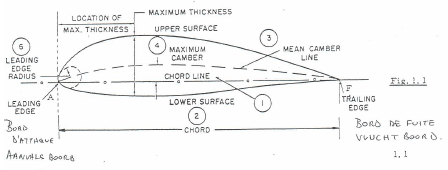
\includegraphics[scale=0.8]{ch2/1}
		\captionof{figure}{}
		\end{center}
		
		The connection between the trailing edge and the leading edge is called the \textbf{chord}. Then we have a \textbf{camber line} which is the line following the shape of the airfoil and characterizing the geometry. The leading and trailing edges are respectively the starting and ending point of the camber line. The thickness is always normal to the camber line. Let's note that the camber line and the thickness distribution are function of the position $f(x)$. \\
		
		Eastman Jacobs created around 1930 a family of wing profiles, known as the NACA profiles. He characterised them by 4 digit numbers: 
		
		\begin{itemize}
			\item[•] The first is the \textbf{maximum camber in percentage of the chord} 
			\item[•] The second is the \textbf{position of the maximum camber in 1/10 percentage of the chord}
			\item[•] The last two digits gives the \textbf{position of the maximum thickness in percentage of the chord}\\
		\end{itemize}				
		
		These were characterizing the 2D representation, but a wing is 3D. We have also the \textbf{wing surface S}, \textbf{the span of the wing b} and we can define a mean chord when this last is not constant as: 
		\begin{equation}
		<c> = \frac{S}{b}.
		\end{equation}				
		 For civil aircraft, b/c is between 6-10 and for glider b/c = 12, this is called the \textbf{aspect ratio} (slenderness ratio). 
		 
		 \newpage
		 
	\section{The flow around 2D airfoils}
		
		\begin{wrapfigure}[9]{l}{7.5cm}
		\vspace{-5mm}
		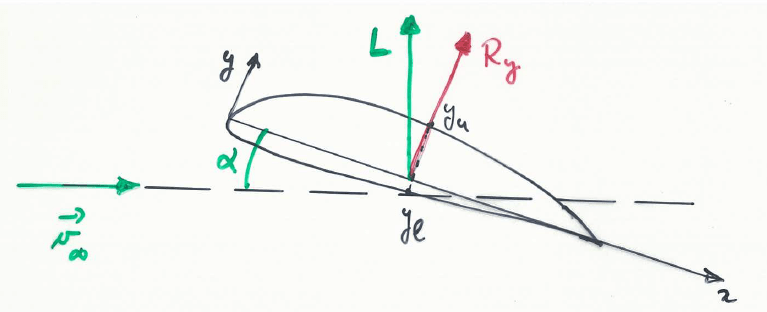
\includegraphics[scale=0.25]{ch2/3}
		\captionof{figure}{}
		\label{fig:2.2}
		\end{wrapfigure}
		Let's remind the expression of the force applied on the wing:
		
		\begin{equation}
		\vec{R} = -\oint p \, d\vec{S} + \oint \bar{\bar{\tau}} \, d\vec{S} 
		\end{equation}
		
		with an external normal to the airfoil. The angle of attack is represented on \autoref{fig:2.2}.

		The pressure term is responsible for lift and the friction term is responsible for drag. Friction forces work tangential to the airfoil and the pressure forces are perpendicular, if there is \textbf{no separation} in the flow. The drag created by the stress is called the \textbf{skin} or \textbf{friction} drag. 
		Note that in a subsonic inviscid incompressible flow, we have the paradox of d’Alembert because we have no drag. This shows that the pressure only contributes to lift. \\

		What happens when we have \textbf{separation} is that we have a region above the airfoil where $p-p_\infty \approx 0$ and so we have a very big pressure below $p\gg p_\infty$ that slows down the wing. This implies that the applied force is higher than the case without separation and due to the attack angle, the drag force too. This phenomenon is called \textbf{pressure drag} (form drag), and here the pressure contributes to drag.
		
		\begin{center}
		ADD FIGURE 4
		\end{center}
		
		\begin{wrapfigure}[15]{r}{6cm}
		\vspace{-5mm}
		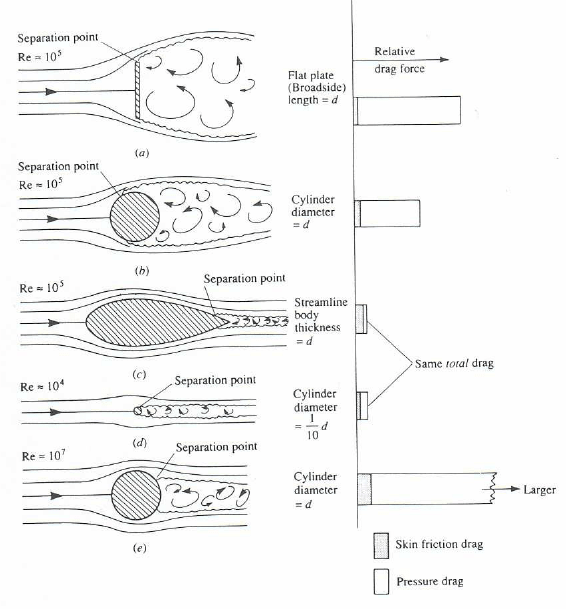
\includegraphics[scale=0.3]{ch2/2}
		\captionof{figure}{}
		\end{wrapfigure}
		The figure shows how the geometry of the body influence the drag force which can be sometimes principally caused by pressure. If we have a flat plate or a cylinder we have a huge separation, so principally a form drag $D_f$. We will have less pressure drop with the wing profile as it perfectly follows the flow direction, to end up smoothly, in this case the friction drag $D_f$ is more important. This shows the importance of profiles. \\
		
		If we look to the weight of a plane, it is surprising to see the importance of lift force. This is possible thanks to the high \textbf{atmospheric pressure}. Indeed, the wing load is defined as: 
		
		\begin{equation}
		\mbox{wing load} = \frac{\mbox{weight plane}}{\mbox{surface aera wings}}
		\end{equation}
				
		and this is commonly approximately equal to 5000 Pa = 500 $kg/m^2$. This can be easely reached by a small perturbation of the atmospheric pressure ($10^5$Pa $\rightarrow$ $5\% = 5000$ Pa). \\
		
		\subsection{Distribution of the pressure coefficient}
			Let's see the effect of the angle of attack. For small angles, we can neglect the force derivation implied and consider it to be perpendicular to the chord. This allows to neglect the drag component (refer to \autoref{fig:2.2}). If we assume that $v$ is in the x direction, the lift force approximation is:
			
			\begin{equation}
			R_y = - \oint p \, d\vec{S}.\vec{1}_y = - \oint p \, dS_y.
			\end{equation}						
			 
			The lift force is fully created by pressure and we can call the lower part of the wing the \textbf{pressure side} and the upper part the \textbf{suction side}. 
			
			\begin{wrapfigure}[11]{l}{8cm}
			\vspace{-5mm}
			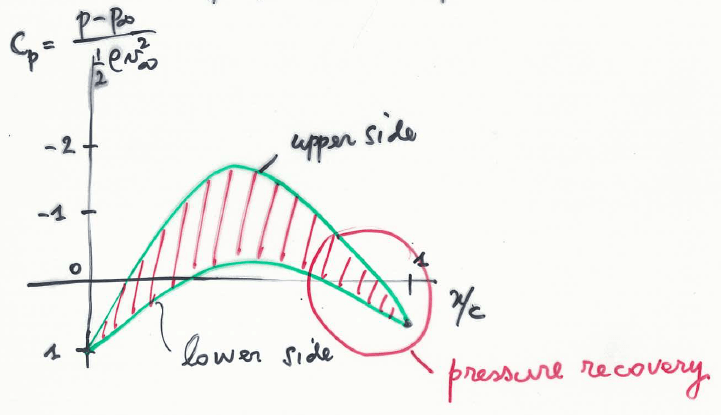
\includegraphics[scale=0.3]{ch2/4}
			\captionof{figure}{}
			\label{fig:2.4}
			\end{wrapfigure}
			The suction effect is always bigger than the pressure one. We introduce the pressure coefficient $C_p = \frac{p-p_\infty}{\frac{1}{2}\rho v_\infty ^2}$ which direction points always down! The pressure side is the green curve below and the suction side is the green curve on the upper side of \autoref{fig:2.4}. \\

			If we look to the leading edge, we have a tendency to go to $C_p = 1$. Indeed, if we write Bernouilli along a streamline and take into account the stagnation point where $v=0$, we have:
			
			\begin{equation}
			p_\infty + \rho \frac{v_\infty ^2}{2} = cst = p_{LE} + 0 \qquad \Rightarrow C_p = \frac{p_{LE}-p_\infty}{\frac{1}{2}\rho v_\infty ^2} = 1.
			\end{equation}						
			
			The pressure recovery means that we will have again $p = p_\infty$ at that point. At the leading edge this is the case because it is commonly a stagnation point. \\ 

For the trailing edge we have two cases. If it is \textbf{blunt} trailing edge, we have the $C_p = 1$ case (leading edge always blunt). If we have a \textbf{sharp} trailing edge, we will have $v_\infty$ at the previous stagnation point and so the Bernouilli equation rewrites:

			\begin{equation}
			p_\infty + \cancel{\rho \frac{v_\infty ^2}{2}} = cst = p_{TE} + \cancel{\rho \frac{v_\infty ^2}{2}} \qquad \Rightarrow C_p = \frac{p_{TE}-p_\infty}{\frac{1}{2}\rho v_\infty ^2} = 0.
			\end{equation}
			
			\begin{wrapfigure}[7]{r}{8cm}
			\vspace{-5mm}
			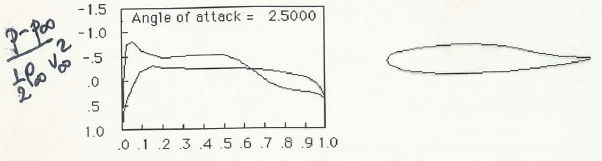
\includegraphics[scale=0.4]{ch2/5}
			\captionof{figure}{}
			\end{wrapfigure}
			We have a very big expansion on the LE (separation), so this induces a suction peak as the pressure falls above and increases below. Then we go back to the normal pressure. Let’s remind that decreasing pressure is favourable because the flow stays attached but if we have pressure increase, it's unfavourable, because we risk separation.
The angle of attack is important because the flow has more difficulties to turn on the LE  when angle goes up so the separation and the sucking peak are more important.\\

			This case is particular because the rear is reversed, so the pressure side becomes sucking and inversely. The reduced camber and reduced thickness makes the wing more vulnerable to angle change.
			
			\begin{wrapfigure}[2]{l}{7.5cm}
			\vspace{-5mm}
			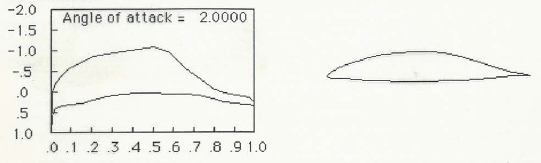
\includegraphics[scale=0.4]{ch2/6}
			\captionof{figure}{}
			\end{wrapfigure}
			Natural laminar section. The smoother LE reduces the peak and the sharp TE induces $C_p = 0$.\\\\
			
			\begin{wrapfigure}[2]{r}{7.5cm}
			\vspace{-5mm}
			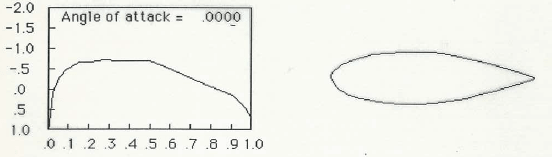
\includegraphics[scale=0.4]{ch2/8}
			\captionof{figure}{}
			\end{wrapfigure}
			This is a symetrical shape and thus only one line is shown. The thickness makes it more resistible to angle change. \\\\\\
			
			\begin{wrapfigure}[2]{l}{7.5cm}
			\vspace{-5mm}
			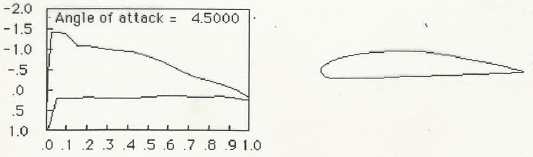
\includegraphics[scale=0.4]{ch2/9}
			\captionof{figure}{}
			\end{wrapfigure}
			Even if the wing is thin, the camber makes it more suited to high attack angle. \\\\\\
		
		\section{Center of pressure, moment and aerodynamic center}
			\subsection{Center of pressure and moment}
				\subsubsection{Calculation of lift force}
					\begin{wrapfigure}[12]{r}{3.5cm}
					\vspace{-5mm}
					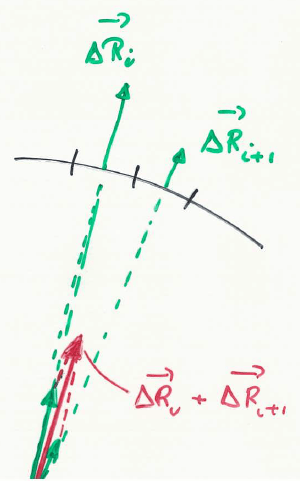
\includegraphics[scale=0.3]{ch2/10}
					\captionof{figure}{}
					\end{wrapfigure}
					We can calculate the lift by $L = \rho v_\infty \Gamma$, but we need the $\Gamma$ which is not calculable. So we will use the trick that consist in forgetting the drag term in the $\vec{R}$. Then we integrate the pressure around the surface:
					
					\begin{equation}
					\vec{R} = -\oint p \, d\vec{S} = - \sum \underbrace{p_i \vec{\Delta S_i}}_{\Delta R_i}
					\end{equation}
					
				\subsubsection{Center of pressure}
					It's the x value on the chord where the carrier of the force $\vec{R}$ intersects the chord. It's function of the angle of attack. Indeed, if alpha increases, the suction peak will be higher, this induces that the center of pressure move forward (participation of the forward pressure more important).\\
					
					Note that the center of pressure is not a fixed point. Indeed, it varies with the angle of attack: if $\alpha \nearrow$, the pressure peak on the LE is more important making the $x_p$ move upstream, and the contrary for $\alpha \searrow$. This notion will be completed by the \textbf{zero lift angle} $\alpha _{0}$.
					
				\subsubsection{Equivalent forces}
					\begin{wrapfigure}[7]{l}{3cm}
					\vspace{-5mm}
					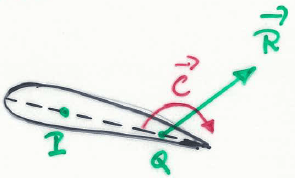
\includegraphics[scale=0.3]{ch2/11}
					\captionof{figure}{}
					\end{wrapfigure}
					The force at the pressure center P is equivalent to another force in point Q, but by adding the moment to compensate the one added by moving the force. This moment is:
					
					\begin{equation}
					\vec{C_Q} = -\vec{PQ}\times \vec{R}.
					\end{equation}
					
				\subsubsection{Aerodynamic center}
					Suppose that there is a point Q where this couple $C_Q$ is independent of the angle of attack (because the pressure center changes with alpha). This point is called the aerodynamic center. We have to show that this exists. For this way:
					\begin{enumerate}
						\item We will begin by calculating the center of pressure by integrating the pressure field. We can calculate the magnitude, but not the acting point. 
						
						\item We compute the momentum of the pressure forces around the leading edge (\autoref{fig:2.11}):
						
						\begin{equation}
						\vec{M}_{LE} = \oint \vec{OQ} \times d\vec{F} = \underbrace{M_{LE}}_{<0} \vec{1}_z 
						\end{equation}
						where $\vec{1}_z$ goes in the paper. 						
						
						\item On the other hand, we know that $\vec{R}$ has a certain direction with a normal component, so we can make the moment (\autoref{fig:2.12}): 
						
						\begin{equation}
						M_{LE} = -x_p.N
						\end{equation}
					\end{enumerate}
					
					By using point 2 and 3 we can find $x_{p}$.
					
					\begin{center}
					\begin{minipage}{0.4\textwidth}
					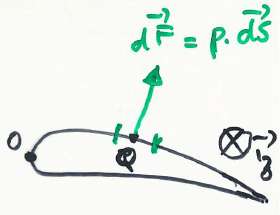
\includegraphics[scale=0.55]{ch2/12}
					\captionof{figure}{}
					\label{fig:2.11}
					\end{minipage}
					\begin{minipage}{0.4\textwidth}
					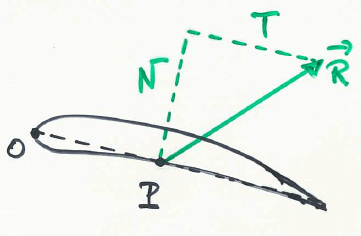
\includegraphics[scale=0.5]{ch2/13}
					\captionof{figure}{}
					\label{fig:2.12}
					\end{minipage}
					\end{center}
					
		\subsection{Aerodynamic center}
			Let's now be interested in how the the moment on a point Q on the wing varies with $\alpha$. It is shown experimentally that:
			
			\begin{equation}
			c_m(Q) = c_{m_0} + k c_l
			\label{eq:2.11}
			\end{equation}
			
			where $c_m, c_l$ are respectively the non-dimensional moment and lift, and $c_{m_0}$ the non-dimensional moment at zero lift. $k$ is a constant that is related to the reference point chosen. If $Q$ is taken on the LE for example, increasing $\alpha$ will produce an increase of the lift and make the center of pressure move upstream. The L increase will compensate the moving $x_p$ such that the moment becomes even more noose-down (more negative following $\vec{1}_z$) $\Rightarrow k<0$ for a decrease in \eqref{eq:2.11}. The same reasoning applied on the trailing edge gives $k>0$. \\
			
			This shows that it exists a point where $k = 0$, called the \textbf{aerodynamic center}. According to \eqref{eq:2.11}, this point will have a constant moment whatever $\alpha$. Indeed, we will show that $c_l = m(\alpha - \alpha _0)$ and so:
			
			\begin{equation}
			c_m(Q) = c_{m_0} + k m(\alpha - \alpha _0) \qquad \Rightarrow c_m(Q) = c_{m_0}.
			\end{equation}			 
			
			We can benefit from this equation to show that $c_{m_0}$ is well the moment for $\alpha = \alpha _0$, the zero lift angle (negative, descending arrow). We will also later show that when we decrease the angle of attack beginning from a positive one to the zero lift angle, the $x_p$ will go downstream till infinity away the trailing edge, with an infinitely small lift,. This means that we will always have a finite noose-down moment. \\
			
			Taking the opposite case of beginning from negative value of $\alpha$, we will have the same value since the lift force is negative and the $x_p$ in infinity further away from the leading edge. The \textbf{moment at zero lift} is thus \textbf{negative}. The explanations lead to the figures below.
			
			\begin{center}
			\begin{minipage}{0.33\textwidth}
			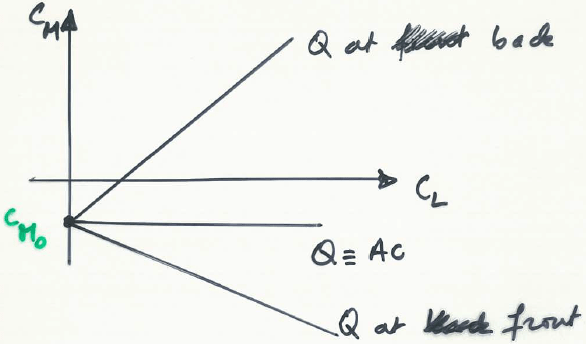
\includegraphics[scale=0.23]{ch2/14}
			\captionof{figure}{}
			\end{minipage}
			\begin{minipage}{0.32\textwidth}
			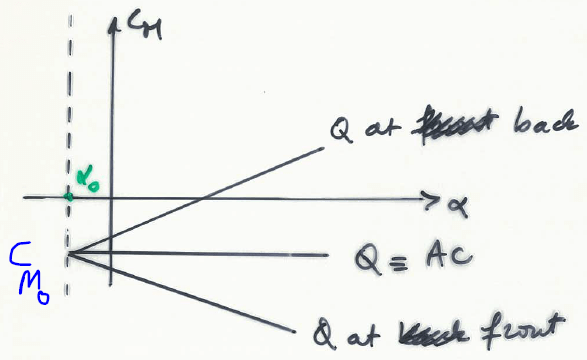
\includegraphics[scale=0.22]{ch2/15}
			\captionof{figure}{}
			\end{minipage}
			\begin{minipage}{0.32\textwidth}
			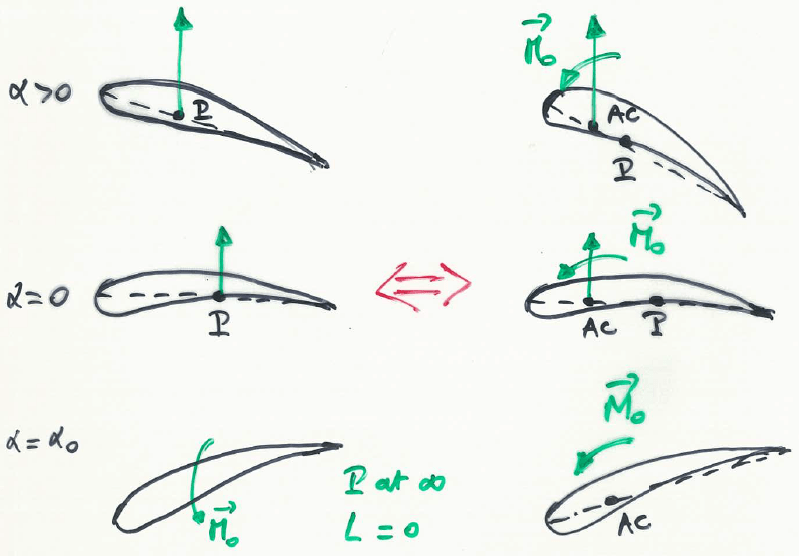
\includegraphics[scale=0.11]{ch2/16}
			\captionof{figure}{}
			\end{minipage}
			\end{center}
		
			\begin{wrapfigure}[8]{l}{4.5cm}
			\vspace{-5mm}
			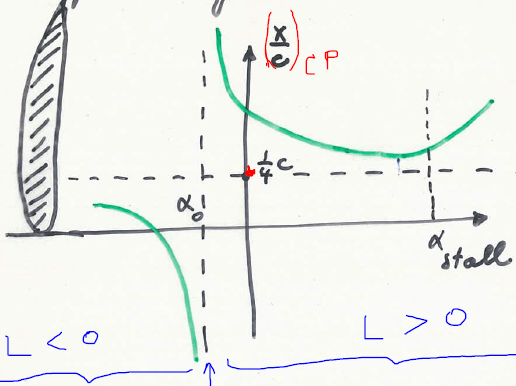
\includegraphics[scale=0.2]{ch2/17}
			\captionof{figure}{}
			\end{wrapfigure}
			Let's finally establish the evolution of the pressure center in function of $\alpha$. For this purpose, we need 4 equations:
			
			\begin{equation}
			\begin{array}{cccc}
			1) & c_m = c_{m_0} + kc_l & 2)& M_{ac} = (x_{ac}-x_{cp})N \\
			3) & m_{ac} = M_{AC} = M_0 <0 & 4) & N = n(\alpha-\alpha _0)
			\end{array}
			\end{equation}
		
		 	The AC being always upstream the CP the difference in 2) is $<0$. In 4), $n>0$. By using equation 3,4 and 2, we can compute:
		 	
		 	\begin{equation}
		 	M_0 = -(x_{cp}-x_{ac}).n(\alpha - \alpha _0) \quad \Leftrightarrow \quad -\frac{M_0}{n} = (x_{cp}-x_{ac}).(\alpha - \alpha _0)
		 	\end{equation}
		 	
		 	This is the equation of an \textbf{hyperbola}. To see it, we only have to compute the limits of:
		 	
		 	\begin{equation}
		 	\begin{array}{c}
		 	x_{cp} = x_{ac} - \frac{M_0}{n}\frac{1}{\alpha - \alpha _0}\\
		 	\lim _{\alpha \rightarrow \pm\infty} x_{cp} = x_{ac} \qquad \lim _{\alpha \rightarrow \alpha _0 >0} x_{cp} = +\infty \qquad \lim _{\alpha \rightarrow \alpha _0 <0} x_{cp} = -\infty
		 	\end{array}
		 	\end{equation}
		 	
		 	The graph is shown on figure. Let's finally say that commonly, $x_{ac} = cst \approx \frac{1}{4}C$.\\
		 	
		 	 A particular case is the one of \textbf{symmetrical profile}. Indeed, in that case, the $\alpha _0$ case correspond to $M_{ac} = 0$ and $L=0$. The pressure center corresponds with the aerodynamic center and is \textbf{fixed}.  
		 	 
	\section{2D characteristics}
		\subsection{Lift, drag and moment curves}
			Let’s look to the non-dimensional parameters that will influence the lift;, the drag and the momentum. We have to define some reference quantities: 

			\begin{equation}
			\begin{array}{cccc}
			L_{ref} = C & v_{ref} = v_\infty & t_{ref} = L_{ref}/v_{ref} & \rho _{ref} = \rho _\infty \\
			t’= t/t_{ref} & p_{ref} = \rho _{ref} \frac{v_{ref} ^2}{2} & \mbox{Mach} = V_{ref} / a_{ref} & a_{ref} = \gamma \pi T_{ref} \\
			\gamma = c_p / c_v && Re_{ref} = \frac{\rho _{ref} v_{ref} L_{ref}}{\mu _{ref}} &
			\end{array}
			\end{equation}					
			
			where $a$ is the speed of sound. By replacing all these in the mass, momentum and energy equations, we obtain the non-dimensional ones (see Fluid Mechanics II):
			
			\begin{equation}
			\begin{aligned}
			&\bullet\frac{\D \rho '}{\D t'} + \nabla \left(\rho ' \vec{v}'\right) = 0\\
			&\bullet\rho ' \frac{d\vec{v}'}{dt'} = - \frac{1}{\gamma M^2_{ref}}\nabla p' + \frac{1}{\mbox{Re}_{ref}}\nabla \bar{\bar{\tau}'}\\
			&\bullet\frac{d}{dt'}(\rho ' e')+ \frac{\gamma (\gamma -1)}{2} M^2_{ref}\frac{d}{dt'}(\rho ' \vec{v'}^2 ) \\
			&= \frac{\gamma}{Pr_{ref}Re_{ref}} \nabla (k'\nabla T') - (\gamma -1)\nabla (p'\vec{v}')+ \gamma (\gamma -1) \frac{M_{ref}^2}{Re_{ref}} \nabla (\bar{\bar{\tau}}'\vec{v}')			\end{aligned}
			\end{equation}
		
			We can see that a solution can only be function of 4 parameters: $M, Re, Pr = \frac{c_p \mu}{k}, \gamma$, but we know that the geometry and the angle of attack $\alpha$ have a role by means of the boundary conditions. Then, we assume that the fluid is air ($\gamma =1.4$) and that we can neglect heat effects (no influence of Pr, incompressible and so low speed flows). The non-dimensional lift, drag and moment are thus function of M, Re, geometry and $\alpha$. We can define \textbf{lift}, \textbf{drag} and \textbf{moment coefficient} as (we forget about compressibility $\rightarrow$ M, and Re effects are low for $C_L and C_M$): 
			
			\begin{equation}
			\begin{aligned}
			&C_L(\cancel{M}, \cancel{Re}, geometry, \alpha) = \frac{L}{\frac{1}{2}\rho _{ref} v^2_{ref} S} \\
			&C_D(\cancel{M},Re, geometry, \alpha) = \frac{D}{\frac{1}{2}\rho _{ref} v^2_{ref} S}		\\
			&C_M(\cancel{M}, \cancel{Re}, geometry, \alpha) = \frac{M}{\frac{1}{2}\rho _{ref} v^2_{ref} Sc}
			\end{aligned}	
			\label{eq:2.18}		
			\end{equation}
			
			where L, D, M are the \textbf{dimensional} forces, c the mean chord (S/b) and S a reference surface (3D wing $\rightarrow$ total wing surface, 2D wing $\rightarrow$ S = c). We can experimentally show that the lift increases mainly linearly with $\alpha$ and the drag force is caused by friction effects and pressure differences involving with $\alpha$. This gives the following equations (lower case for 2D):
			
			\begin{equation}
			c_l = m(\alpha - \alpha _{L_0}) \qquad c_d = c_{d_0} + kc^2_l
			\end{equation}
			
			where $m\approx 2\pi$ theoretically and 5.7 practically, k is a constant of order of magnitude 0.01. 
			
		\subsection{Stall and critical angle of attack}
			\begin{wrapfigure}[11]{l}{6cm}
			\vspace{-5mm}
			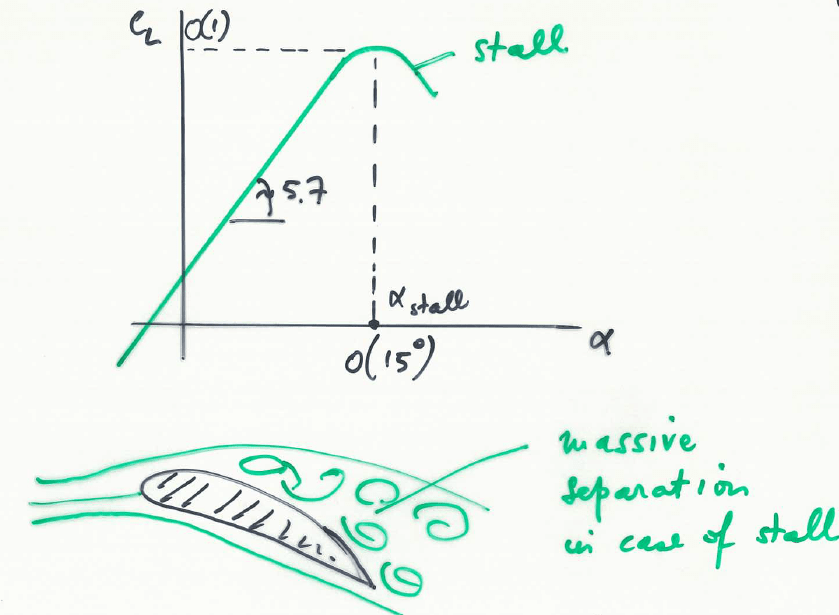
\includegraphics[scale=0.16]{ch2/18}
			\captionof{figure}{}
			\end{wrapfigure}
			At a certain angle of attack ($\approx 15\degres$), the lift suddenly drops. This is due to massive separation on the suction side (reverse pressure gradient too high) and happens at the \textbf{critical angle of attack}. This phenomenon is called \textbf{stall}. In the separated part, the pressure will no longer decrease and will form a pressure plateau. \\
			
			We have to make the difference between leading-edge stall and trailing-edge stall. For \textbf{leading-edge stall}, the massive separation occurs suddenly near the LE resulting \newpage
			
			\begin{wrapfigure}[13]{r}{5.7cm}
			\vspace{-5mm}
			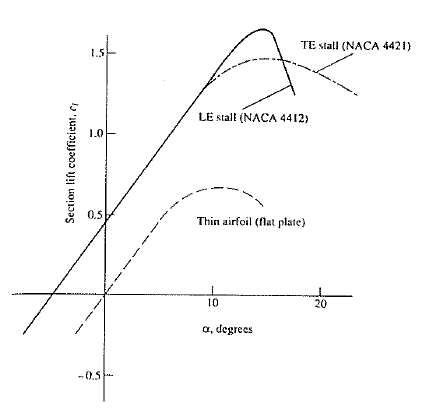
\includegraphics[scale=0.4]{ch2/19}
			\captionof{figure}{}
			\end{wrapfigure}
			in a strong and sudden drop of lift, when at maximum lift. This especially occurs to thin airfoils with cross-sections between 10 and 16\% of the chord. For the \textbf{trailing-edge stall}, the point of separation gradually goes upstream with increasing angle of attack resulting in a more gradual drop of lift (more thick airfoils). The comparison is done on the right figure. We can also see a third type of stall called \textbf{thin airfoil stall} with the example of a flat plat.  \\
			
			In conclusion, the LE must be sufficiently rounded to have a good maximum lift. In fact the profile may nor be too 
			
			\begin{wrapfigure}[8]{l}{7cm}
			\vspace{-5mm}
			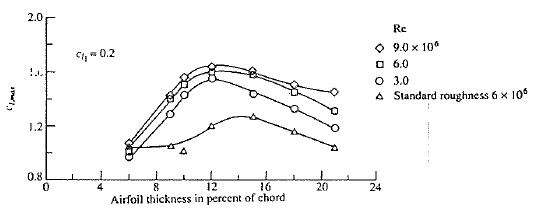
\includegraphics[scale=0.4]{ch2/20}
			\captionof{figure}{}
			\end{wrapfigure}
			thick  nor too thin. The figure on the left shows the influence of the thickness on the lift. We notice that the optimum thickness is situated around 12\% of the chord.The maximum lift increases with RE, indeed higher the Re, higher is the ratio of speed versus viscosity. So we can better oppose to separation. Unlike the Re number, the roughness has great effects on the maximum lift. Finally, let's notice that the camber have also an effect on maximum lift, the best is a camber of 8 up to 10\%. 
			
		\subsection{Maximum lift, stalling speed, polar curve and glide ratio}
			From $C_L$ in \eqref{eq:2.18}, we can deduce the lift:
			
			\begin{equation}
			L = C_L \frac{1}{2} \rho _{ref} v^2_{ref} S.
			\label{eq:2.21}
			\end{equation}
			
			The lift force must always at least be equal to the weight of the plane. This implies that for low speed (take-off and landing), the $C_L$ must be large. This is accomplished with large $\alpha$ and slats or flaps. The minimum speed where the lift can still balance the weight ($C_L$ maximum) is called \textbf{stall speed} and from \eqref{eq:2.21} we find:
			
			\begin{equation}
			v_{stall} = \sqrt{\frac{W}{C_{L_{max}} \frac{1}{2} \rho_{ref} S}}
			\end{equation}
			
			\begin{wrapfigure}[10]{r}{4cm}
			\vspace{-5mm}
			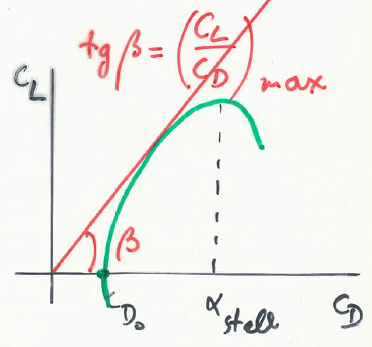
\includegraphics[scale=0.3]{ch2/21}
			\captionof{figure}{}
			\end{wrapfigure}
			The curve that represents $C_L$ in function of $C_D$ is the \textbf{polar curve} of the wing. The ratio $\frac{C_L}{C_D}$ is the \textbf{glide ratio} or \textbf{finesse} and is like an efficiency parameter. The best parameter is obtained using the graph by calculating $\beta$ such that: 
			
			\begin{equation}
			\tan \beta = \left(\frac{C_L}{C_D}\right)_{max}
			\end{equation}						
			 
			This point is important for the quality of the wing because if we plot the thrust, the lift, the drag and the weight of a plane describing a horizontal flight (\autoref{fig:2.21}), the thrust is given by:
			
			\begin{equation}
			T = \frac{L}{\tan \beta} = \frac{W}{\tan \beta}
			\end{equation}
			
			where we see that when $\tan \beta$ (so the glide ratio) increases, T decreases. Another interpretation can be given when we have no thrust (\autoref{fig:2.22}). In this case the gliding ratio has to be adapted to travel the larger distance knowing that:
			
			\begin{equation}
			\frac{C_L}{C_D} = \frac{\mbox{distance travelled}}{\mbox{height loss}}
			\end{equation}
			
			\begin{center}
			\begin{minipage}{0.3\textwidth}
			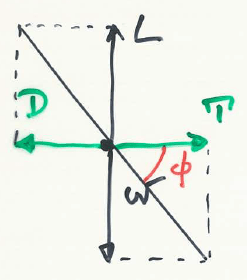
\includegraphics[scale=0.5]{ch2/22}
			\captionof{figure}{}			
			\label{fig:2.21}
			\end{minipage}
			\begin{minipage}{0.5\textwidth}
			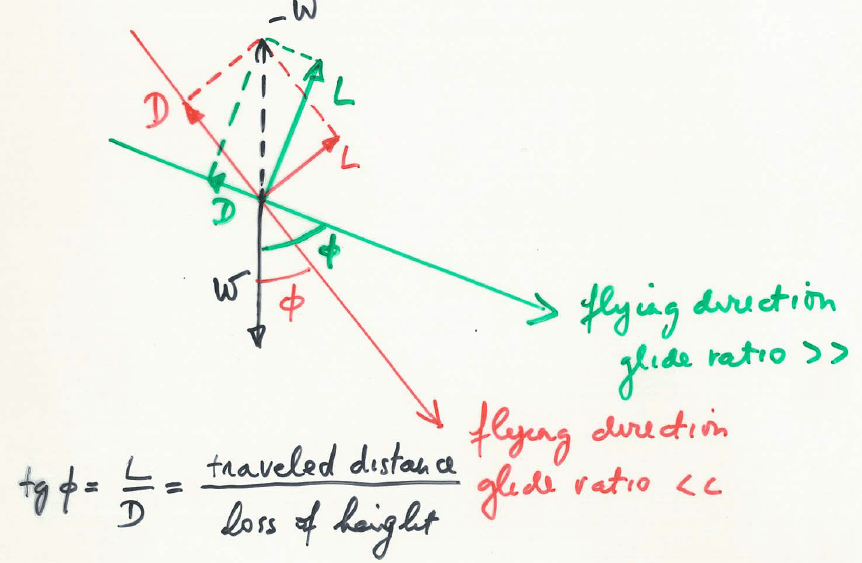
\includegraphics[scale=0.2]{ch2/23}
			\captionof{figure}{}			
			\label{fig:2.22}
			\end{minipage}
			\end{center}
			
\section{Methods to calculate flows around 2D airfoils}
	\subsection{Conformal mapping}
		We will begin here with steady, inviscid irrotational flows. This gives for the mass conservation equation:
		
		\begin{equation}
		\frac{\D \rho}{\D t} + \nabla (\rho \vec{v}) = 0 \qquad \Rightarrow \nabla \vec{v} = 0 = \D _x u + \D _y v
		\end{equation}
		
		In the other hand, we have the assumption of irrotational flow:
		
		\begin{equation}
		\vec{\omega} = 0 \qquad \Rightarrow \D _x v - \D _y u = 0.
		\end{equation}
		
		Then we define the \textbf{complex potential function w}:
		
		\begin{equation}
		w = \phi + I\psi
		\end{equation}		 
		
		where $\phi$ is the \textbf{potential function} (satisfies $w=0$ by construction) such that:
		
		\begin{equation}
		\left\{
		\begin{aligned}
		&u = \D _x \phi \\
		&v = \D _y \phi
		\end{aligned}
		\right.
		\qquad
		\nabla \phi = \vec{v} = \D _x\phi \vec{1} _x + \D _y \phi \vec{1}_y
		\end{equation}
		
		We must satisfy the mass conservation equation:
		\begin{equation}
		\nabla (\nabla \phi) = 0 \qquad \Rightarrow \Delta \phi = 0 
 		\end{equation}
 		
 		coupled with boundary conditions, we can find a solution $\phi (x,y)$. The \textbf{stream function} satisfies the mass conservation by construction:
 		
 		\begin{equation}
 		\left\{ 
 		\begin{aligned}
 		&u = \D _y \psi\\
 		&v = - \D _x \psi
 		\end{aligned}
 		\right.
 		\qquad \Rightarrow \D _x u + \D _y v = 0 \Leftrightarrow \D _x (\D _y \psi) + \D _y (- \D _x \psi) = 0
 		\end{equation}
 		
 		\begin{wrapfigure}[8]{l}{4cm}
		\vspace{-5mm}
		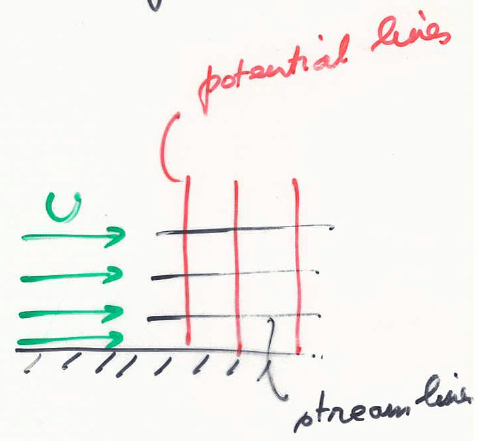
\includegraphics[scale=0.2]{ch2/24}
		\label{fig:2.23}
		\captionof{figure}{}
		\end{wrapfigure}
		We still have to verify the $\omega=0$ condition:
 		\begin{equation}
 		\D _x v - \D _y u = 0 \qquad \Rightarrow \frac{\D ^2 \psi}{\D x^2} + \frac{\D ^2 \psi}{\D y^2} = 0 \qquad \Delta \psi = 0
 		\end{equation}
 		A streamline and a potential line are perpendicular to each other:
 		\begin{equation}
 		\nabla \psi . \nabla \phi = \D _x \psi \D _x \phi + \D_ y \psi \D _y \phi = -vu + uv = 0. 
 		\end{equation}
 		
 		
 	\subsubsection{Theory of analytical functions}
 		Analytical means differentiable. This consist in defining a function $f(z)$ analytical such that:
 		
 		\begin{equation}
 		 w = f(z) \qquad z,\omega \in \mathbb{C} \qquad \Rightarrow w = \phi +i \psi \qquad \left\{
 		 \begin{aligned}
			&z= x+iy\\ 		 
			&\phi = \phi (x,y) \in \mathbb{R}\\
			&\psi =  \psi(x,y) \in \mathbb{R}
\end{aligned} 		  
 		 \right.
 		\end{equation}
 		
 		If this is differentiable everywhere, $\Delta \phi = \Delta \psi = 0$. We have a way to determine the complex velocity (velocity field):
 		
 		\begin{equation}
 		\frac{dw}{dz} = \frac{df}{dz} = A + iB \qquad A = \frac{\D \phi}{\D x} = - \frac{\D \psi}{\D y} = u \quad B = \frac{\D \psi}{\D x} = - \frac{\D phi}{\D y} = -v
 		\end{equation}
 		
 		A property of this $f(z)$ is the superposition principle: $w_1 = f_1(z), w_2 = f_2(z)$ so $w_1 + w_2 = f_1(z)+f_2(z)$.
 		
 	\subsubsection{Uniform flow}
 		This case corresponds to \autoref{fig:2.23}:
 		\begin{equation}
 		w = U z \qquad \frac{d w}{dz} = U = u+iv \qquad \Rightarrow u = U; v = 0
 		\end{equation}
 		
 	\subsubsection{Source / Sink}
 		\begin{wrapfigure}[8]{r}{3cm}
		\vspace{-5mm}
		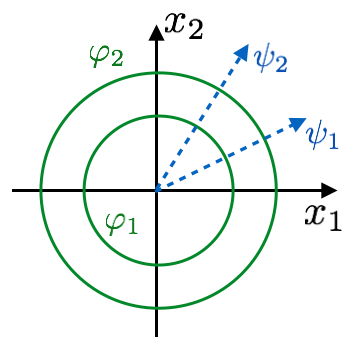
\includegraphics[scale=0.3]{ch2/25}
		\captionof{figure}{}
		\end{wrapfigure}
		In this case, using the cylindrical coordinates, the complex potential is defined as ($\Lambda$ being the volumetric flow): 
 		
 		\begin{equation}
 		\begin{aligned}
 		&w = \frac{\Lambda}{2\pi} \ln z = \frac{\Lambda}{2\pi} \ln (r e^{i\theta}) = \frac{\Lambda}{2\pi} (\ln r + i\theta) \\
 		&\Rightarrow \phi = \frac{\Lambda}{2\pi} \ln r, \psi =  \frac{\Lambda}{2\pi}\theta.
 		\end{aligned}
 		\end{equation}
 		
 		We see that complex lines corresponds to $r =cst$ so are circles and streamlines $\theta = cst$ are line of constant angle. $\oint \vec{v}\, d\vec{l}=0$ as velocity is everywhere tangent to any circular contour. Let's compute the derivative for the velocity field:
 		
 		\begin{equation}
 		\frac{dw}{dz} = \frac{\Lambda}{2\pi z} = \frac{\Lambda (x-iy)}{2\pi (x^2+y^2)} = \frac{\Lambda}{2\pi r} (\cos \theta - i \sin \theta).
 		\end{equation}
 		
 		We see that the velocity decreases in $1/r$, this is due to the constant mass flow, so if the surface increases with r the velocity has to decrease to keep $\dot{m} = \rho v S$ constant. 
 		
 	\subsubsection{Free vortex}
 		\begin{wrapfigure}[5]{l}{3cm}
		\vspace{-5mm}
		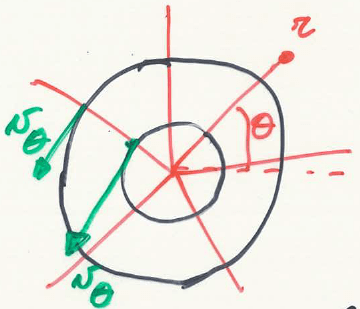
\includegraphics[scale=0.23]{ch2/26}
		\captionof{figure}{}
		\end{wrapfigure}
		We do the same as the other cases: 
 		\begin{equation}
 		\begin{aligned}
 		&w = \frac{i\Gamma}{2\pi} \ln z = \frac{i\Gamma}{2\pi} \ln (re^{i\theta}) = \frac{i\Gamma}{2\pi} (\ln r + i\theta) = -\frac{\Gamma}{2\pi} \theta + \frac{i\Gamma}{2\pi} \ln r \\
 		&\phi = -\frac{\Gamma}{2\pi} \theta, \psi = \frac{\Gamma}{2\pi} \ln r
 		\end{aligned}
 		\end{equation}
 		
 		We see that this is the inverse case of the previous one, streamlines are circles oriented in negative rotational motion around z-axis (z entering tin the sheet) so clockwise. We can compute the velocity field by deriving among z and we find that: 
 		
 		\begin{equation}
 		u = \frac{\Gamma \sin \theta}{2 \pi r} \qquad v = -\frac{\Gamma \cos \theta}{2\pi r}
 		\end{equation}
 		
 		Let's specify that $v_\theta = \frac{1}{r} \frac{\D \phi}{\D \theta} = -\frac{\Gamma}{2 \pi r}$, and that we have a vortex singularity in the center because $\Gamma = 0. \infty$.
 		
 	\subsubsection{Flow around a cylinder}
 		\begin{wrapfigure}[5]{r}{5.5cm}
		\vspace{-5mm}
		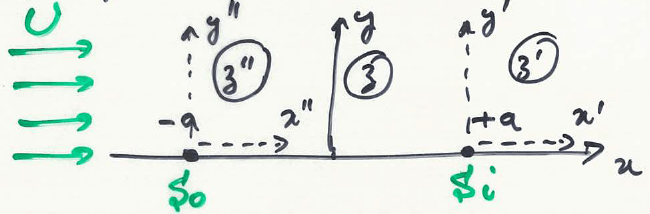
\includegraphics[scale=0.23]{ch2/27}
		\captionof{figure}{}
		\end{wrapfigure}
		Let's make a combination of a uniform flow and a source + sink as shown on the figure. The combination gives:
		
		\begin{equation}
		w = Uz + \frac{\Lambda}{2\pi} \ln \frac{z+a}{z-a}= Uz + \frac{\Lambda}{2\pi} \ln \frac{1+a/z}{1-a/z}.
		\end{equation}
		
		To have the flow around a cylinder we need to compute the limit $a\rightarrow 0$, and will need the Taylor expansion of $\ln$:
		
		\begin{equation}
		\ln \frac{1+\epsilon}{1-\epsilon} \approx 2 \epsilon + \cancel{o(\epsilon ^3)} \qquad \Rightarrow \lim _{a\rightarrow 0} w = \lim _{a \rightarrow 0} \left[ Uz + \frac{\Lambda}{2\pi} 2 \frac{a}{z} \right]
		\end{equation}
		
		by defining $\mu = 2\Lambda a$ we find the \textbf{flow around a cylinder}:
		
		\begin{equation}
		w = Uz + \frac{\mu }{2\pi z}.
		\label{eq:2.42}
		\end{equation}
		
		If we replace $z= x+iy$ to find $\phi$ and $\psi$ we find:
		
		\begin{equation}
		\phi = Ux + \frac{\mu}{2\pi }\frac{x}{r^2} \qquad \psi = Uy - \frac{\mu }{2\pi} \frac{y}{r^2}.
		\end{equation}
		
		In this flow a closed streamline exists forming the so called \textbf{Rankine body} and which describes a cylinder in the case $a\rightarrow 0$. Indeed it is possible to find an exact solution for $\psi = 0$. This configuration has a symmetry according to x and y-axis when taking the center of the cylinder as origin. This implies that $\vec{F} = - \oint _{cyl} p\, d\vec{S} = 0$. This is the so called \textbf{paradox of d'Alembert} because we expect to find at least a drag force. A lift force can be find on the cylinder by adding a vortex. We conclude by saying that we can rewrite \eqref{eq:2.42} as (R the radius of the cylinder):
		
		\begin{equation}
		w = U\left( z + \frac{R^2}{z} \right) \qquad with \ R^2 = \frac{\mu }{2\pi U}.
		\end{equation}
		
		\newpage
		
	\subsubsection{Cylinder Joukowski transformation}
		\begin{wrapfigure}[5]{l}{5.5cm}
		\vspace{-5mm}
		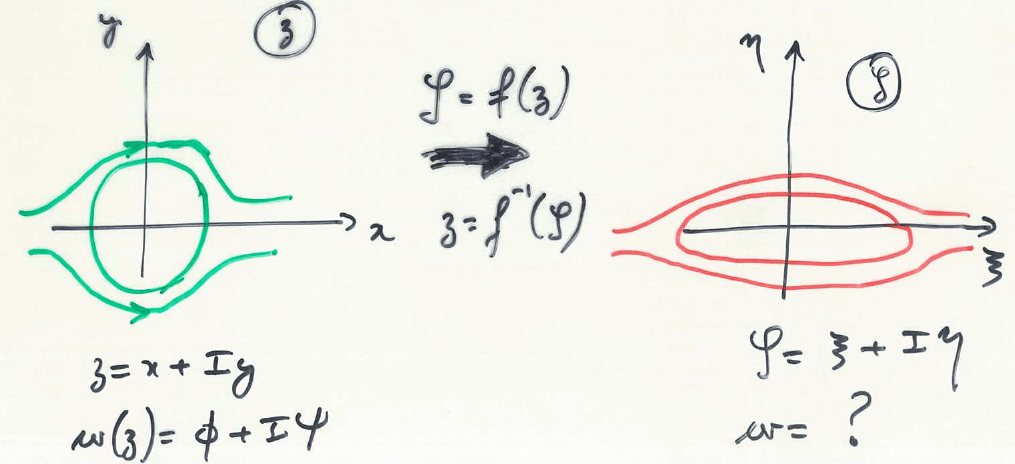
\includegraphics[scale=0.1]{ch2/28}
		\captionof{figure}{}
		\end{wrapfigure}
		Let's do a mapping, a transformation, to try to find our airfoil based on simple geometries. Let's as first example apply the transformation $Z = z + \frac{R^2}{z}$ to the cylinder of radius R. Let's first remark that the cylinder will become a flat plate:
		
		\begin{equation}
		Z = z + \frac{R^2}{z} = Re^{i\theta}  \frac{R^2}{Re^{i\theta}} = 2 R \cos \theta 
		\end{equation}
		
		Indeed, as $\cos \theta \in [-1,1]$ and the result is real, we have a flat plate between -2R and 2R in the x-axis. The flow Z is directly found: $W(Z) = UZ$. The second example will be the application of the same transformation on a cylinder of this time radius $r>R$. In this case the circle becomes an ellipse:
		
		\begin{equation}
		Z = r e^{i\theta} + \frac{R^2}{r^2}e^{-i\theta} = \left( r + \frac{R^2}{r} \right)\cos \theta + i \left( r - \frac{R^2}{r} \right) \sin \theta.
		\end{equation}		 
		
		Let's also compute the velocity field using the chain rule:
		
		\begin{equation}
		\frac{dW}{dZ} = \frac{dw}{dZ} = \frac{dw}{dz}\frac{dz}{dZ} = \left( 1 -\frac{r^2}{z^2} \right) \left( \frac{1}{1-\frac{R^2}{z^2}} \right).
		\end{equation}
		
		We see that the expression becomes infinite when $z^2 = R^2$. The reason is that the transformation is not analytical in these points so they must not be in the flow. 
		
		The examples are summarized in the figures below 
		
		\begin{center}
		\begin{minipage}{0.45\textwidth}
		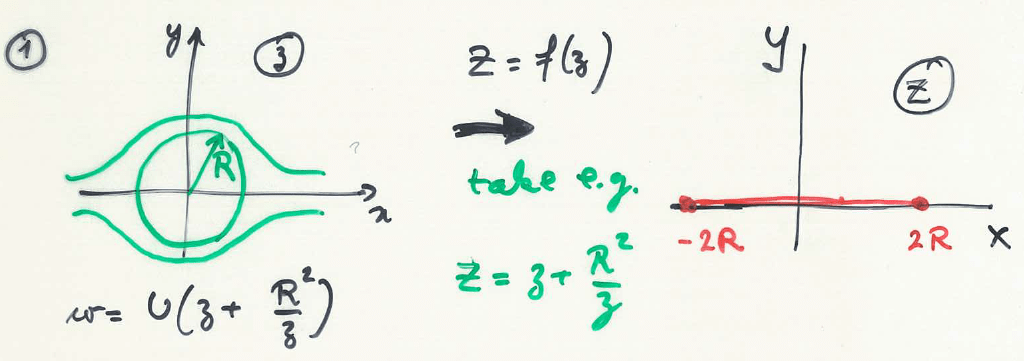
\includegraphics[scale=0.15]{ch2/29}
		\captionof{figure}{}
		\end{minipage}
		\begin{minipage}{0.45\textwidth}
		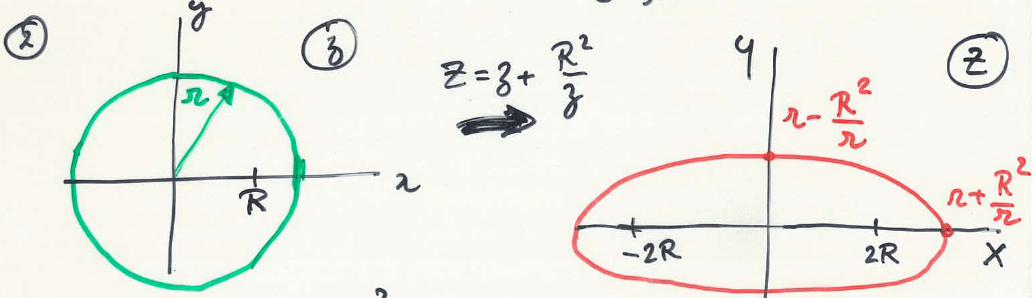
\includegraphics[scale=0.2]{ch2/30}
		\captionof{figure}{}
		\end{minipage}
		\end{center}
		
		Now suppose that we place no longer the center of the cylinder at the origin, but on the real axis. The mapping of the cylinder now takes the shape of a \textbf{symmetrical wing profile}. We see that there is two remarkable points that are H and A corresponding to the points $H_1$ and $A_1$ of the black and red circles, our profile is in between them. Now to give camber we only have to move the center of the cylinder on the y-axis. Please reffer to figures below. 
		
		\begin{center}
		\begin{minipage}{0.45\textwidth}
		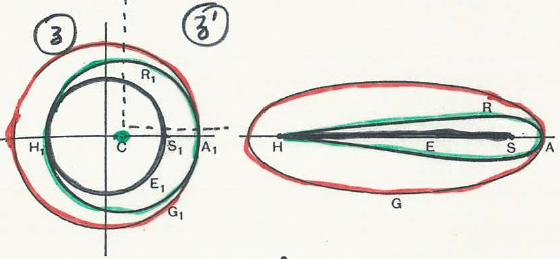
\includegraphics[scale=0.3]{ch2/31}
		\captionof{figure}{}
		\end{minipage}
		\begin{minipage}{0.45\textwidth}
		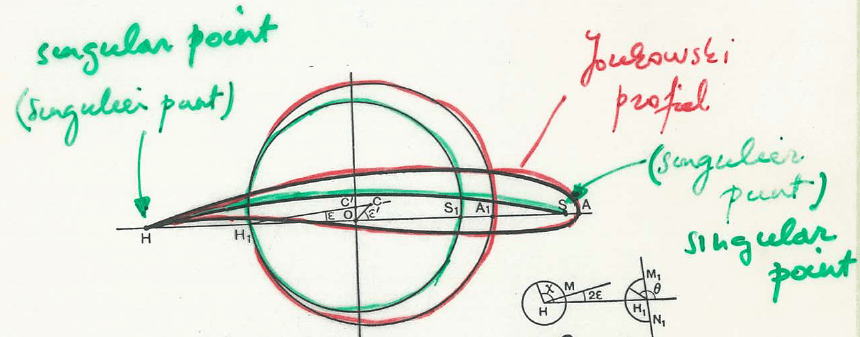
\includegraphics[scale=0.2]{ch2/32}
		\captionof{figure}{}
		\end{minipage}
		\end{center}
		
		Note that for the green circle in first figure, the complex potential becomes:
		
		\begin{equation}
		w = U\left( z-z_c + \frac{r^2}{z-z_c} \right)
		\end{equation}
		
		As last remark, let's remind that we had singularities in the second example. These points corresponds here to $H_1$ and $S_1$. The mapping of $H_1$ is always H the trailing edge, the velocity is there infinitely large. This was the discussion we've previously done with the stagnation point that has to move on the trailing edge otherwise $v = \infty$ because of the sharp edge. We can solve this by adding a vortex. This methods gives a limited amount of airfoils. 
		
\subsection{Thin airfoil theory}
	We will suppose infinitely thin airfoil and small angle of attack, so that the airfoil is represented by the camber line. This means also small camber about 2-3\% of the chord and $\alpha <8\%$. We can try to retrieve the flow by superposition principle by using infinite number of elementary sources or elementary vorticies. The potential function for the source and the elementary one are:
	
	\begin{equation}
	\phi = \frac{\Lambda}{2\pi} \ln r \qquad d\phi = \frac{d\Lambda}{2\pi} \ln r
	\end{equation}		
	
	We then describe the source distribution by the source intensity $\lambda = \frac{d\Lambda}{ds}$ on a part $ds$ of the wing so that the last equation becomes:
	
	\begin{equation}
	d\phi = \frac{\lambda}{2\pi} \ln r\, ds.
	\end{equation}
	
	We will use the second method presented now which is using the vorticies: 
	
	\begin{equation}
	\phi = -\frac{\Gamma}{2\pi} \theta \qquad \vec{v} = \nabla \phi = \underbrace{\frac{\D \phi}{\D r} \vec{1}_r}_{= v_r = 0} + \underbrace{\frac{1}{r} \frac{\D \phi}{\D \theta} \vec{1} _\theta}_{= v_\theta} \qquad \Rightarrow v_\theta = -\frac{\Gamma }{2\pi} \frac{1}{r}.
	\end{equation}
	
	In the same way as the other we can define a \textbf{vortex intensity} to characterize the vortex distribution on a part ds $\gamma = \frac{d\Gamma}{ds}$, the derivative of $\phi$ and the elementary velocity are then: 
	
	\begin{equation}
	d\phi = -\frac{\gamma}{2\pi} \theta \, ds \qquad dv_\theta = -\frac{\gamma ds}{2\pi r}.
	\end{equation}
	
	The aim now is to make that infinitely thin airfoil a streamline, but which distribution of $\gamma$ is needed? To compute this, we can assume because of superposition that the flow is a uniform flow $\vec{U}_\infty$. We also assume that we have an angle of attack $\alpha$. Because of the vorticies, we have a velocity perturbation $\vec{v}$ such that the total velocity is: 
	
	\begin{equation}
	\vec{V}_\infty = \vec{U}_\infty + \vec{v}.
	\end{equation}
	
	\begin{wrapfigure}[9]{l}{8.5cm}
	\vspace{-5mm}
	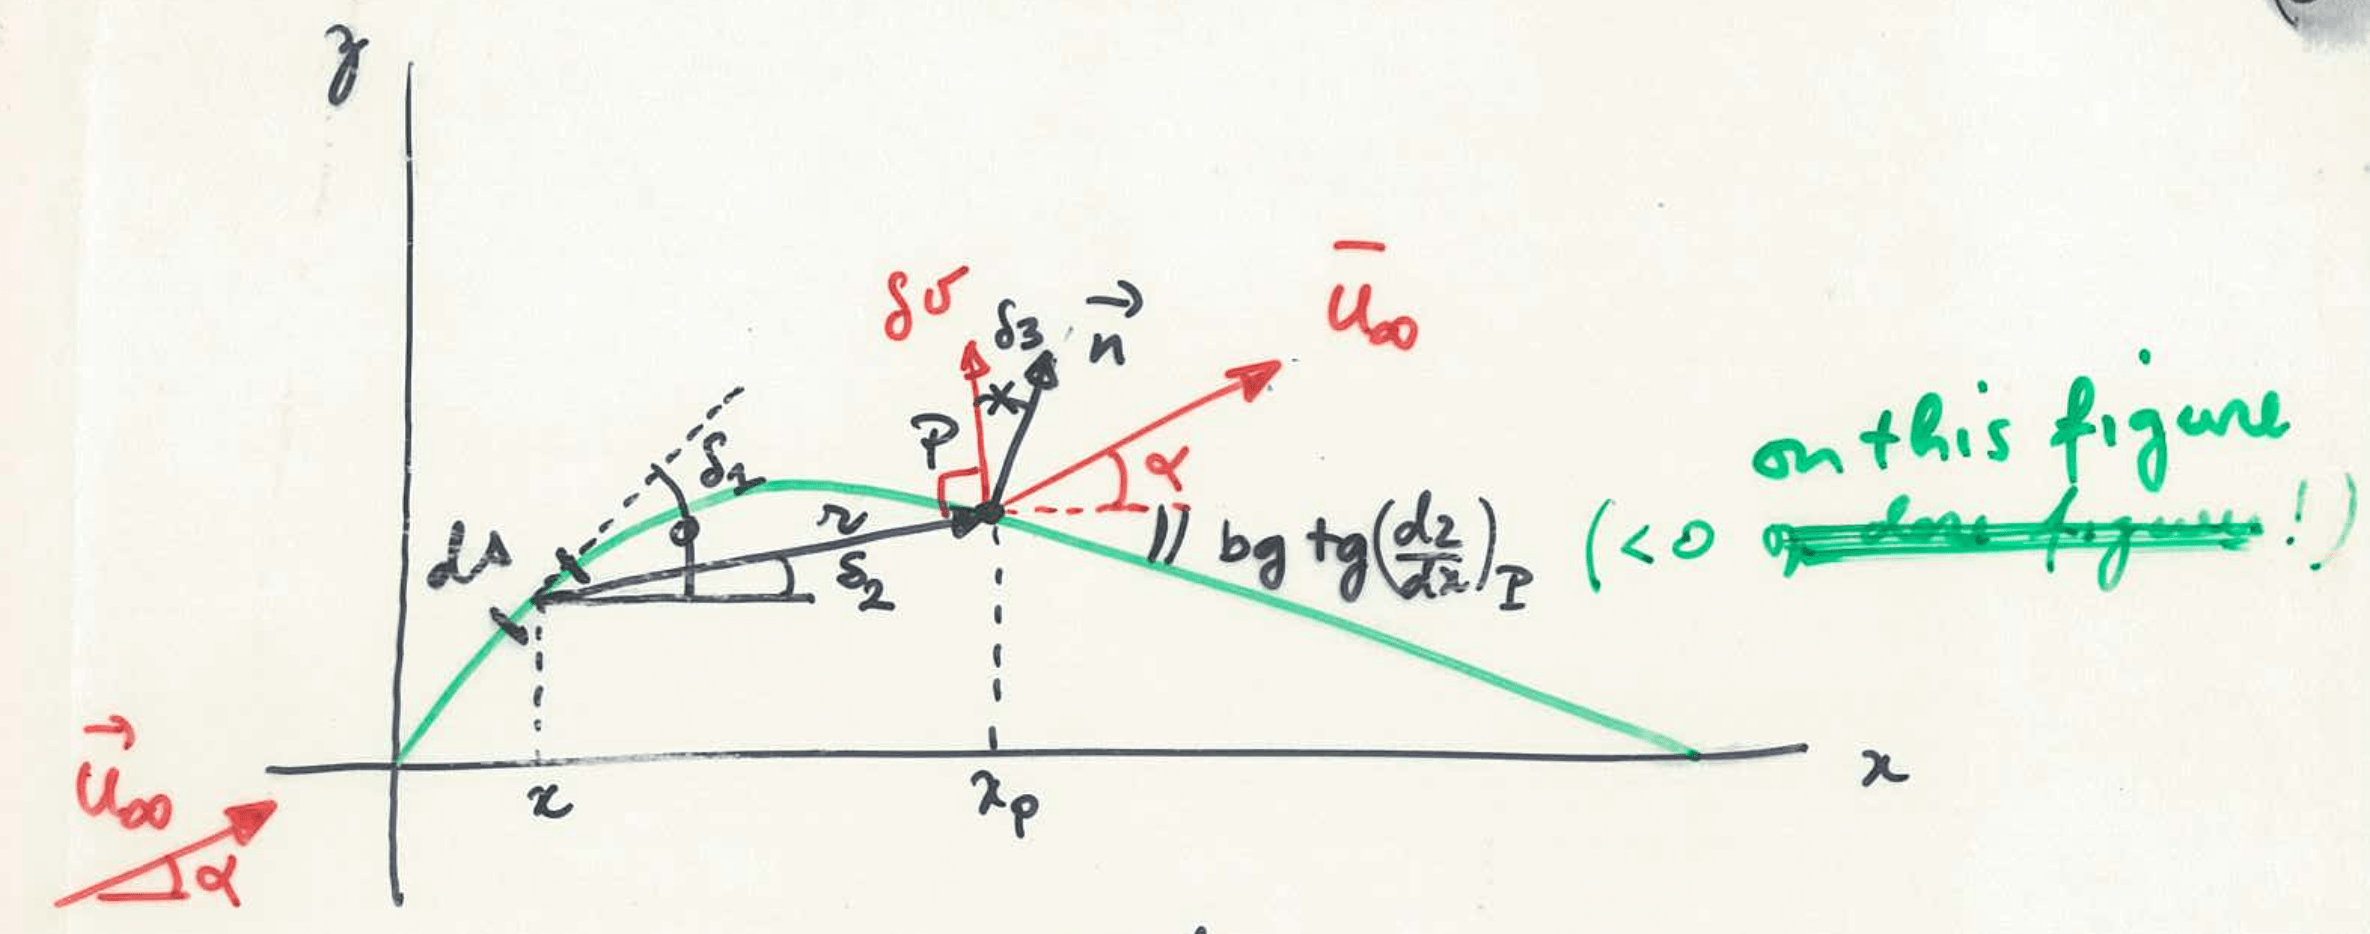
\includegraphics[scale=0.1]{ch2/33}
	\captionof{figure}{}
	\end{wrapfigure}
	We must now choose $\gamma$ such that $\vec{V}$ is tangential to the airfoil everywhere (we want the camber line to be a streamline). In other words, $\forall P$ the normal component of the velocity should be null $V_{nP} = U_{\infty _{nP}} + v_{nP} = 0$. Let's determine these components by projection. First, for $U_{\infty _{nP}}$ we can remark the sum of angle $\alpha$ and the camber line slope $\tan \beta =  \left(-\frac{dz}{dx}\right)_p \Rightarrow \beta = -\arctan \left(\frac{dz}{dx}\right)_p$, the projection is (camber line: $z = f(x)$):
	
	\begin{equation}
	U_{\infty _{nP}} = U_\infty \sin \left[ \alpha - \arctan \left(\frac{dz}{dx} \right)_P \right].
	\label{eq:2.54}
\end{equation}	 

	Now for $v_{np}$, we consider an elementary vortex on a point $x$ on the airfoil that creates an elementary perturbation $\delta v_n$ on point P. This velocity direction is $\theta$ in a $(r,\theta)$ axis with origin at x, so perpendicular to r on the figure. If the angle with the normal is $\delta _3$, the projection will be:
	
	\begin{equation}
	\delta v_n = -\frac{\gamma (x) ds}{2\pi r} \cos \delta _3 .
	\end{equation}
	
	Now we have infinite number of contribution of the infinite vorticies, as $\gamma , r$ and $\delta _3$ depends on position $P$, we have to integrate over the whole airfoil:
	
	\begin{equation}
	v_n = - \frac{1}{2\pi }\int _0 ^c \frac{\gamma (x) ds}{r} \cos \delta _3
	\end{equation}
	
	where $c$ is the chord length. We can express both $r$ and $ds$ in function of x as: 
	
	\begin{equation}
	r = \frac{x_P - x}{\cos \delta _2} \qquad ds = \frac{dx}{\cos \delta _1}
	\end{equation}
	
	which gives 
	\begin{equation}
	v_n = - \frac{1}{2\pi }\int _0 ^c \frac{\gamma (x) dx}{x_P - x} \frac{\cos \delta _2}{\cos \delta _1}\cos \delta _3. 
	\end{equation}
	
	We are able to reconsider the condition \eqref{eq:2.54} by replacing our results: 
	
	\begin{center}
	\theor{
	\begin{equation}
	\frac{1}{2\pi }\int _0 ^c \frac{\gamma (x) dx}{x_P - x} \frac{\cos \delta _2}{\cos \delta _1}\cos \delta _3 =  U_\infty \sin \left[ \alpha - \arctan \left(\frac{dz}{dx} \right)_P \right].
	\end{equation}
	}
	\end{center}
	
	This is a relatively complicated equation, we can simplify it by \textbf{assuming a small camber} (in practice 2\% of the chord), which allows to say that $\delta _1 \approx \delta _2 \approx \delta _3 \approx 0$ and $\arctan \left( \frac{dz}{dx}\right) _P = \left( \frac{dz}{dx}\right) _P$. By considering $\alpha$ small, $\sin \alpha \approx \alpha$:
	
	\begin{equation}
	\frac{1}{2\pi} \int _0 ^c \frac{\gamma (x)\, dx}{x_P - x} = U_{\infty}\left[ \alpha -  \left(\frac{dz}{dx} \right)_P \right].
	\end{equation}
	
	We will introducce a new variable $\theta$ and not anymore decribe the system using $x$ by considering $x = \frac{1}{2}c (1-\cos \theta)$ and $dx = \frac{1}{2}c \sin \theta\, d\theta$: 
	
	\begin{equation}
	\frac{1}{2\pi} \int _0 ^{\pi} \frac{\gamma (\theta)\sin \theta \, d\theta}{\cos \theta - \cos \theta _P} = U_{\infty}\left[ \alpha -  \left(\frac{dz}{dx} \right)_P \right].
	\label{eq:2.61}
	\end{equation}
	
	This is a quite difficult equation, so let's complicate it even more by expressing $\gamma (\theta )$ in series: 
	
	\begin{equation}
	\gamma (\theta ) = 2U_\infty \left(A_0 \coth \frac{\theta }{2} + \sum _{n=1}^\infty) A_n \sin (n\theta)\right).
	\end{equation}
	
	This is in fact a solution of the last equation but we will not demonstrate it. Notice simply that this respects the Kutta condition that states that there is no vortex allowed on the trailing edge. Indeed for $\gamma (\pi) = 0$  which means no contribution by vortex. We can also state that at the leading edge, the stagnation point is in the pressure side at the front. Indeed, for $\theta = 0$, $\coth \theta = \infty = \gamma (\pi )$ which means that we have a singularity at the TE and that the velocity is infinite due to the turning on the LE.  \\
	
	Now we can replace this definition on the previous equation, knowing that $\coth (\theta /2) \sin \theta = 1+\cos \theta$ and renoting $\theta _P = \theta '$, we get:
	
	\begin{equation}
	\frac{1}{2\pi} \int _0 ^{\pi} \frac{\gamma (\theta)\sin \theta \, d\theta}{\cos \theta - \cos \theta _P}  = \frac{U_\infty}{\pi} \left[ \int _0 ^{\pi} \frac{A_0 (1+\cos \theta ) \, d\theta}{\cos \theta - \cos \theta '} + \sum _n A_n \int _0 ^{\pi}  \frac{\sin (n\theta)\sin \theta \, d\theta}{\cos \theta - \cos \theta '}  \right]
	\end{equation}
	
	By using the equality here and the \textbf{Glauert integral}:
	
	\begin{equation}
	\sin (n\theta ) \sin \theta = - \frac{1}{2} [\cos [(n+1)\theta] - \cos [(n-1)\theta]] \qquad \int _0 ^\pi \frac{\cos (n\theta)\, d\theta}{\cos \theta - \cos \theta '} = \pi \frac{sin(n\theta ')}{sin \theta '}
	\end{equation}
	
	The integral becomes: 
	
	\begin{equation}
	\frac{U_\infty}{\pi} \left[ A_0.0 + A_0. \pi - \frac{\pi}{2} \sum _n A_n \frac{\sin [(n+1)\theta '] - \sin [(n-1)\theta ']}{\sin \theta '} \right] = U_\infty \left[ A_0 - \sum _n A_n \cos (n\theta ') \right]
	\end{equation}
	
	where we used the simpson equation. The \eqref{eq:2.61} becomes: 
	
	\begin{center}
	\theor{
	\begin{equation}
	A_0 - \sum _n A_n \cos (n\theta ') = \alpha - \left( \frac{dz}{dx} \right)'
	\end{equation}
	}
	\end{center}
	
	This equation must be valid $\forall P$ on the airfoil. To find the coefficients $A_i$, let's integrate first this for $0\leq \theta ' \leq \pi$ in order to compute $A_0$: 
	
	\begin{equation}
	A_0\pi - \cancel{\sum _n A_n \int _0 ^\pi \cos (n\theta ')d\theta '} = \alpha\pi - \int _0 ^\pi \frac{dz}{dx}d\theta\qquad \Rightarrow A_0 = \alpha - \frac{1}{\pi} \int _0^\pi \frac{dz}{dx}\, d\theta.
	\end{equation}
	
	For the $A_n$, we multiply the same equation by $\cos (m\theta ')$ before integrating (we will drop the '). Let's see that $\int _0 ^\pi \cos (n\theta)\cos (m\theta) d\theta = 0$ if $ m \neq n $ and $= \pi /2$ if $n = m$. We finally get:
	
	\begin{equation}
	A_n = \frac{2}{\pi} \int _0 ^\pi \frac{dz}{dx} \cos (m\theta) \, d\theta .
	\end{equation}
	
	We can note that for $A_n$ only the camber plays a role, the angle of attack does not appear. Only $A_0$ is influenced by $\alpha$. We are now able to compute any vorticity distribution $\gamma (\theta)$, for example for a flat plate $A_n = 0$ and $A_0 = \alpha$. 
	
\subsubsection{Calculation of the total circulation}
	To get $\Gamma$ we only have to compute the integral over the whole airfoil:
	
	\begin{equation}
	\begin{aligned}
	\Gamma &= \int _0 ^c \gamma (x) \, dx = \frac{1}{2} c \int _0 ^c \gamma (\theta ) \sin \theta \, d\theta \\
	& = \frac{1}{2} c \left[ 2U_\infty \int _0 ^\pi A_0 (1+\cos\theta) \, d\theta + 2U_\infty \sum _{n=1}^\infty \int _0^\pi A_n \sin (n\theta)\sin \theta \, d\theta  \right] \\
	&= U_\infty  c \left[  A_0 \pi  + 2U_\infty + \int _0^\pi \sin ^2(\theta) \, d\theta - \frac{1}{2} \sum _{n=2}^\infty \cancel{\int _0^\pi A_n \cos [(n+1)\theta - \cos (n-1)\theta ] \, d\theta } \right] \\
	&= U_\infty c [A_0 \pi + A_1 \pi /2].
	\end{aligned}
	\end{equation}
	
	We see that the circulation only depends on two coefficients. 
	
\subsubsection{Calculation of the lift coefficient}
We can now compute the lift using the kutta formula $L = \rho _\infty U_\infty \Gamma$. We are interested in the $c_l$ and not the lift itself. In 2D we have to divide by the chord so: 
	
	\begin{equation}
	c_l = \frac{L}{\frac{1}{2} \rho _\infty U_\infty ^2 C} = \frac{2\Gamma}{U_\infty c} = \pi (2A_0 + A_1)
	\label{eq:2.70}
	\end{equation}
	
	We can now replace by definition of the coefficients: 
	
	\begin{equation}
	c_l = 2\pi\left(\alpha - \underbrace{\frac{1}{\pi} \int _0^\pi \frac{dz}{dx} (1-\cos \theta)\, d\theta}_{\alpha _0} \right) = 2\pi (\alpha - \alpha _0)
	\label{eq:2.71}
	\end{equation}
	
	where $\alpha _0$ is the \textbf{zero lift angle of attack}. We see that we have a linear relation with respect to $\alpha$. We have the theoretical model the same for every profile, only $\alpha _0$ changes with the profile. Remark that the lift is also the integral of the pressure on the lower and upper side:
	
	\begin{equation}
	L = \int _0 ^c (p_l - p_u) \, dx = \rho _\infty U_\infty \int _0 ^c \gamma \, dx \qquad \Rightarrow p_l - p_u = \rho _\infty U_\infty \gamma (x).
	\end{equation}
	
\subsubsection{Calculation of the momentum at the leading edge}
	\begin{wrapfigure}[5]{l}{4.5cm}
	\vspace{-5mm}
	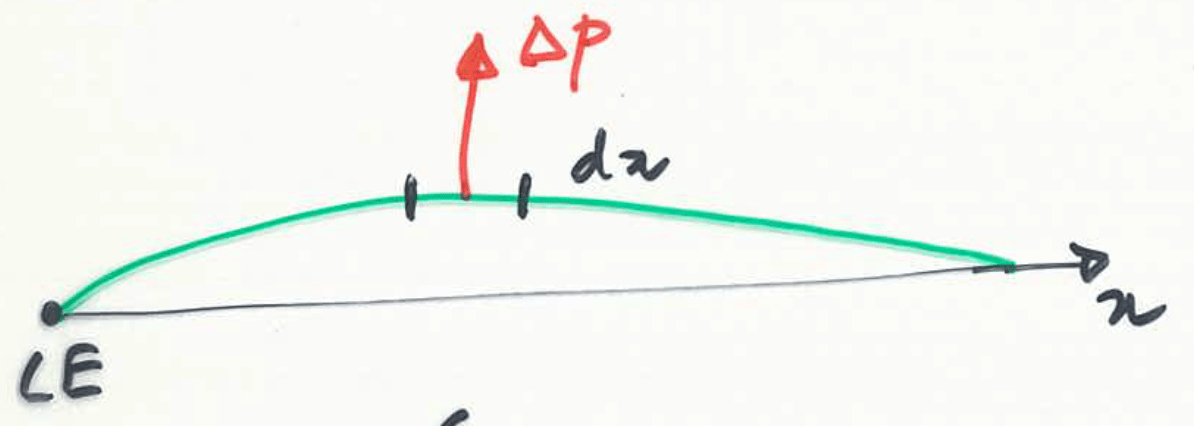
\includegraphics[scale=0.1]{ch2/34}
	\captionof{figure}{}
	\end{wrapfigure}
	The contribution of the elementary parts of the airfoil gives:
	
	\begin{equation}
	\begin{aligned}
	&dM_{LE} = - (\Delta p \, dx) x \\ 
	\Rightarrow &M_{LE} = -\int _0 ^c \Delta p x \, dx = - \rho _\infty U_\infty \int _0^c \gamma x \, dx
	\end{aligned}
	\end{equation}
	
	After some manipulations (not detailed):
	
	\begin{equation}
	c_{m_{LE}} = \frac{M_{LE}}{\frac{1}{2}\rho _\infty U_\infty ^2 c^2} = - \frac{\pi}{4} (2A_0 + 2A_1 - A_2) = -\frac{1}{4} c_l - \frac{\pi}{4} (A_1 - A_2)
	\end{equation}
	
	where we used \eqref{eq:2.70} for the last expression. This is of the same shape than \eqref{eq:2.11} with negative k. 
	
\subsubsection{The aerodynamic center}
	\begin{wrapfigure}[6]{l}{4.5cm}
	\vspace{-5mm}
	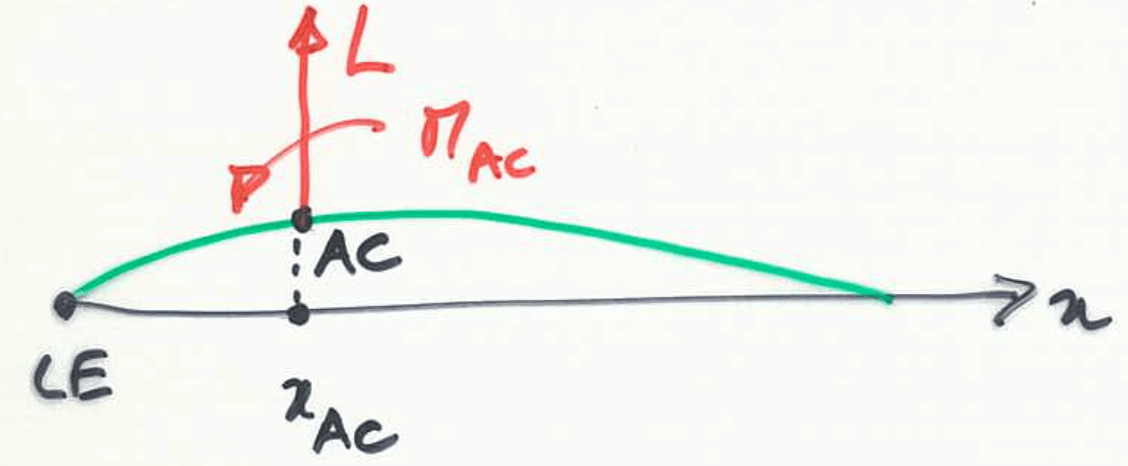
\includegraphics[scale=0.1]{ch2/35}
	\captionof{figure}{}
	\end{wrapfigure}
	The moment on the LE is related to the moment anywhere:
	
	\begin{equation}
	M_{LE} = M_{ac} - x_{ac} L \qquad \Rightarrow c_{m_{LE}} =c_{m_{ac}} - \frac{x_{ac}}{c}c_{l} 
	\end{equation}
	
	By using the last result of the previous section, we get: 
	
	\begin{equation}
	c_{m_{ac}} = \left( \frac{x_{ac}}{c} - \frac{1}{4} \right) c_l - \frac{\pi}{4} (A_1 -A_2).
	\end{equation}
	
	We see that, for this relation to be independent of the angle of attack, we must have $x_{ac} = \frac{c}{4}$ so that: 
	
	\begin{equation}
	c_{m_{ac}} = \frac{\pi}{4} (A_2 - A_1).
	\label{eq:2.77}
	\end{equation}
	
	Remark that for symmetrical wings $\frac{dz}{dx} = 0 \Rightarrow A_1 = A_2 = 0 \Rightarrow c_{m_{ac}} = 0$. 
	
\subsubsection{Calculation of center of pressure}
	The formula used in the previous section is valid, we replace ac by cp, and since the moment should be null at this point:
	
	\begin{equation}
	c_{m_{cp}} = c_{m_{LE}} + \frac{x_{cp}}{c} c_l = 0 \qquad \Rightarrow \frac{x_{cp}}{c} = \frac{1}{4} + \frac{\frac{\pi}{4}(A_1-A_2)}{c_l} = \frac{1}{4} - \frac{c_{m_{ac}}}{c_l}.
	\end{equation}
	
	Some remarks: 
	
	\begin{itemize}
	\item[•] the center of pressure is not fixed and varies with the lift
	\item[•] at 0 lift, $x_{cp}\rightarrow \infty$ (for symmetric wing $x_{cp} = x_{ac} = c/4$ fixed)
	\item[•] cp always downstream to ac because $c_{m_{ac}}<0$.
	\end{itemize}
	
\subsubsection{Effect of flaps}
	\begin{wrapfigure}[5]{l}{4.5cm}
	\vspace{-5mm}
	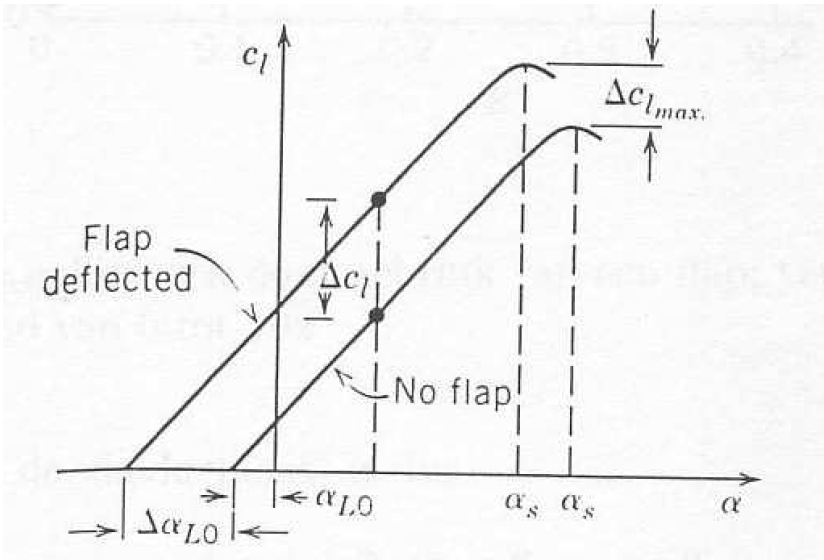
\includegraphics[scale=0.1]{ch2/36}
	\captionof{figure}{}
	\end{wrapfigure}
	According to the definition of the zero lift angle in \eqref{eq:2.71}, the effect of the shape becomes greater when $\theta \approx 180\degres$ (trailing edge). By making the zero lift angle more negative we can produce more lift before the critical angle of attack that decreases a bit. 
	
	\ \\\\\\
	
	\begin{wrapfigure}[6]{r}{3.5cm}
	\vspace{-5mm}
	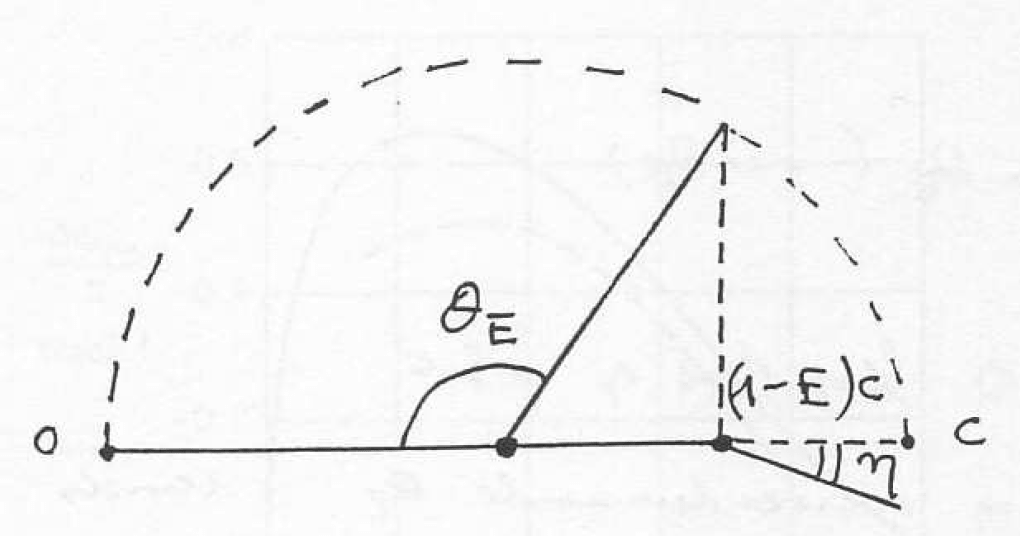
\includegraphics[scale=0.1]{ch2/37}
	\captionof{figure}{}
	\end{wrapfigure}
	The effect is evaluated by taking a flat plate as camber line with a deflection near the TE, starting at E\% of the chord and slope $\eta$. E in function of $\theta _E$ is: 
	
	\begin{equation}
	E = \frac{1}{2} (1+\cos \theta _E).
\end{equation}	 

	In this case, $A_0$ and $A_n$ can be rewritten as:
	
	\begin{equation}
	\begin{aligned}
	&A_0 = \alpha - \frac{1}{\pi} \int _0 ^\pi \frac{dz}{dx} d\theta \approx \alpha - \frac{\eta}{\pi} (\pi - \theta _E) \\
	&A_n = \frac{2}{\pi} \int _0 ^\pi \frac{dz}{dx} \cos (n\theta )d\theta \approx -\frac{2\eta}{\pi} \frac{1}{n} \sin (n\theta _E)
	\end{aligned}
	\end{equation}
	
	such that the lift coefficient becomes: 
	
	\begin{equation}
	c_l = \pi (2A_0 + A_1) = \underbrace{2\pi \alpha}_{\mbox{without flaps}} \underbrace{- 2\eta (\pi - \theta _E + \sin \theta)}_{\Delta c_l > 0 \mbox{ since } \eta < 0}.
	\end{equation}
	
	This seams to be like $c_l = 2\pi (\alpha - \alpha _0)$ allowing the definition for the zero lift angle: 
	
	\begin{equation}
	\alpha _0 = \frac{\eta}{\pi} (\pi - \theta _E + \sin \theta)
	\end{equation}
	
	which indicates an increase (decrease since $\eta <0$) of $\alpha _0$ since it is null for the flat plate. For the moment at the ac \eqref{eq:2.77}
	
	\begin{equation}
	\Delta c_{m_{ac}} = \frac{\eta }{2} \sin \theta _E (1- \cos \theta _E)
	\end{equation}
	
	which also indicates a decrease in the momentum which is 0 for the symmetric wing. 
	
	\begin{wrapfigure}[3]{l}{4cm}
	\vspace{-5mm}
	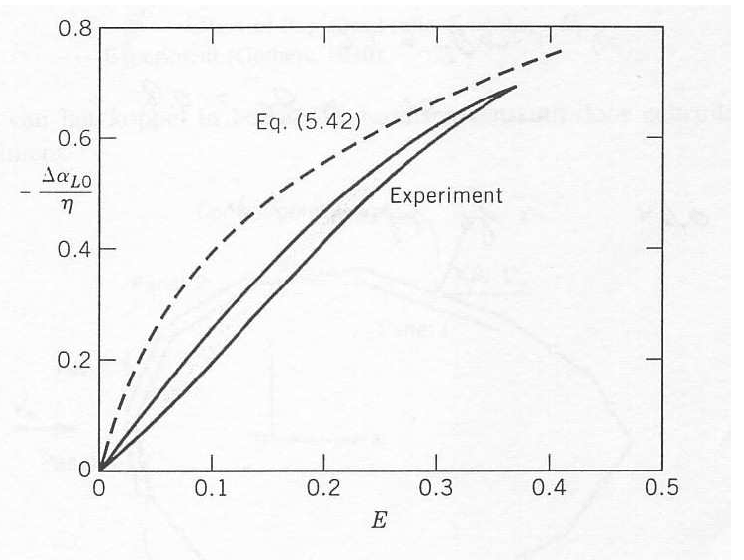
\includegraphics[scale=0.1]{ch2/38}
	\captionof{figure}{}
	\end{wrapfigure}
	Here is plotted the the modification of $\alpha _0$ by the flaps. The theory is quite good except for small E (near the TL). This is due to the fact that the flap is immersed into the boundary layer in this region. 
	\ \\\\\\


\subsection{Numerical methods: source panel and vortex panel}
\subsubsection{Source panel}

	\begin{center}
	\begin{minipage}{0.4\textwidth}
	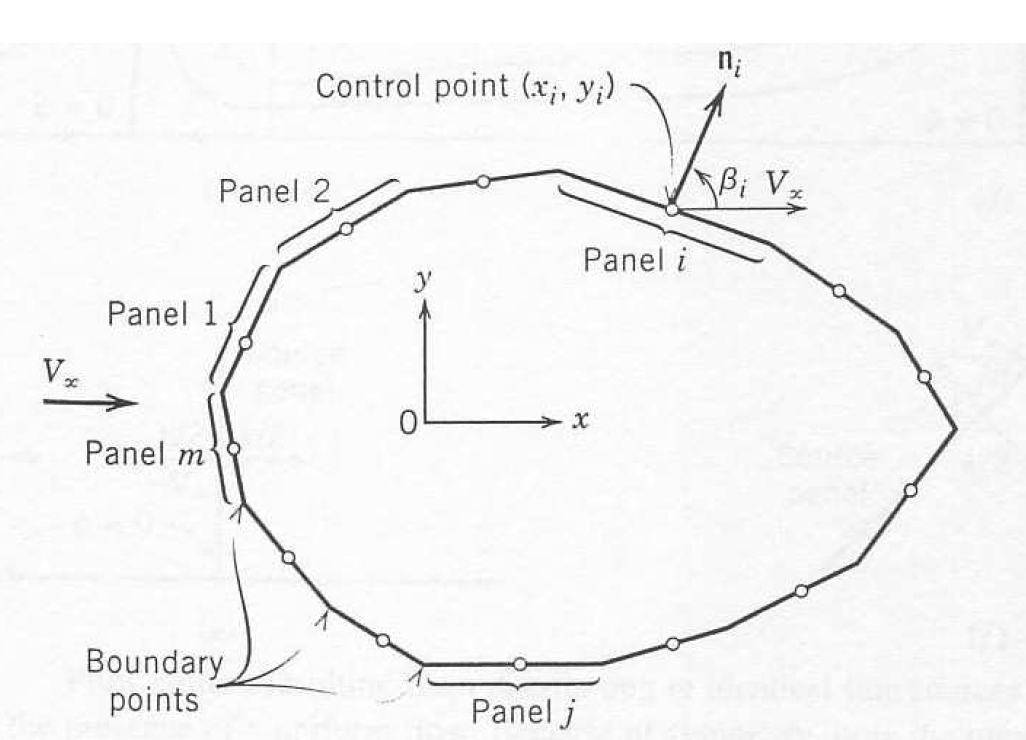
\includegraphics[scale=0.15]{ch2/39}
	\captionof{figure}{}
	\end{minipage}
	\begin{minipage}{0.4\textwidth}
	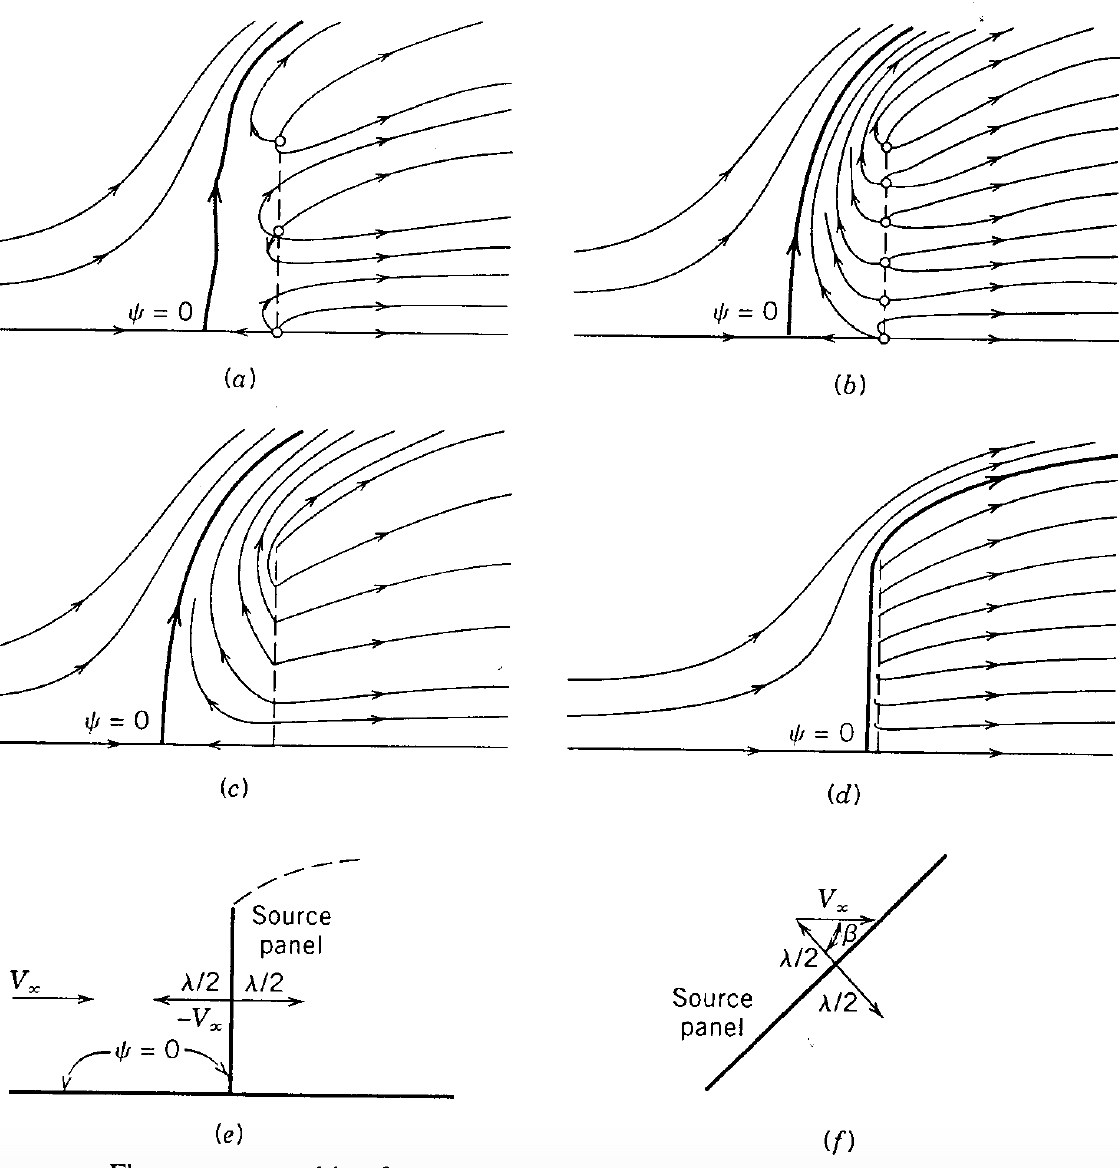
\includegraphics[scale=0.15]{ch2/40}
	\captionof{figure}{}
	\end{minipage}
	\end{center}
	The method consists in subdividing the geometry into panels that each contains a source with source intensity $\lambda _j =\frac{d\Lambda _j}{ds_j}$, where $d\Lambda _j$ is the elementary volumetric flow rate associated to the part $ds_j$. The second figure illustrates the panel concept. We can see the flow obtained by placing sources on a vertical line. From a to d the number of sources increases but the total flow remains the same (d reduced flow rate). \\
	
	Using an infinite number of sources and a constant $\lambda$, we obtain a panel in e. Remark that the velocity is perpendicular to the plate in that case. \\
	
	Next we have to write the potential function and express that the flow should be tangential to the plate. Remark that since there is no vortex the lift is null. 
	
	\begin{wrapfigure}[8]{l}{7cm}
	\vspace{-5mm}
	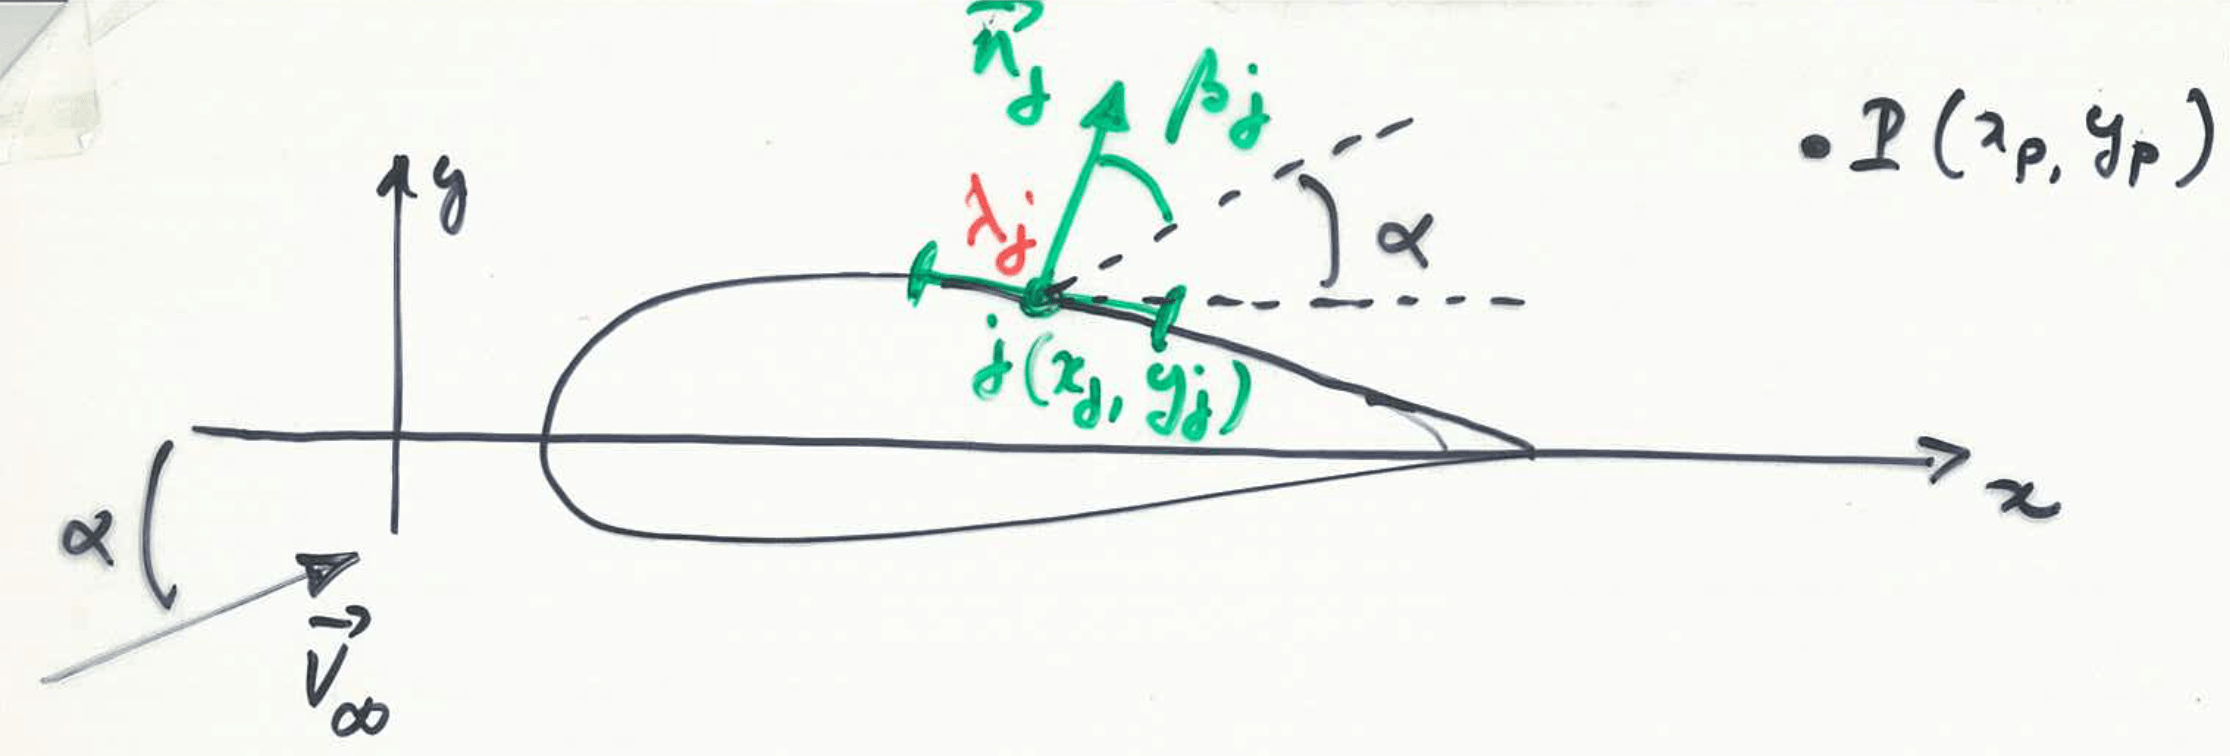
\includegraphics[scale=0.08]{ch2/41}
	\captionof{figure}{}
	\end{wrapfigure}
	Consider the airfoil here and let's write the potential function for the uniform flow at point P:
	
	\begin{equation}
	\phi _{uP} = U_\infty \cos \alpha x + U_\infty \sin \alpha y
	\end{equation}
	 
	 On the other hand, the source distribution on panel j also generates a potential function:
	 
	 \begin{equation}
	 \phi _{jP} = \int _{\mbox{panel } j} \frac{\lambda _j}{2\pi} \ln (r_{jP})ds_j\qquad r_{jP} = \sqrt{(x_P - x_j)^2 + (y_P - y_j)^2}.
	 \end{equation}
	 
	 The total potential is the sum of all that and all the panels j. The condition for the flow to be tangential to panel i is $\frac{\D \phi}{\D n_j} = 0$. This applied to our total potential gives (P is the control point of the panel i):
	 
	 \begin{equation}
	 U_\infty \cos \beta _i + \sum _j \frac{\lambda _j}{2\pi} \int _{\mbox{panel }j} \frac{\D}{\D n_i} (\ln (r_{ji})) \, ds_j = 0,
	 \end{equation}
	 
	 where $\lambda _j$ is assumed to be constant on panel j. The integral regroups the effect of panel j on the normal component of the velocity on panel i, this is only function of the geometry! Note that even if the effect of panel i on its own component leads to $r_{ji} = r_{ii} = 0$ (singular integral), one can show that:
	 
	 \begin{equation}
	 \int _{\mbox{panel }i} \frac{\D}{\D n_i} (\ln (r_{ii})) \, ds_i = \pi,
	 \end{equation}
	 
	 so that the contribution of the panel i is reduced to $\lambda /2$, reducing the general equation to: 
	 
	 \begin{equation}
	 U_\infty \cos \beta _i +\frac{\lambda}{2}+ \sum _{j\neq i} \frac{\lambda _j}{2\pi} \int _{\mbox{panel }j} \frac{\D}{\D n_i} (\ln (r_{ji})) \, ds_j = 0.
	 \end{equation}
	 
	 Since this is a system of N equation in N unknowns (N panel), we are able to find every $\lambda _i$. Using again the potential function, we are able to get now the tangential velocity at panel i: 
	 
	 \begin{equation}
	 v_{ti} = \frac{\D \phi}{\D s_i} = U_\infty \sin \beta _i + \sum _j \frac{\lambda _j}{2\pi} \int _{\mbox{panel }j} \frac{\D}{\D s_i} (\ln (r_{ji})) \, ds_j .
	 \end{equation}
	 
	 Since a panel i only generates a normal velocity, it has no effect on its own tangential velocity, we can show that: 
	 
	 \begin{equation}
	 \int _{\mbox{panel }i} \frac{\D}{\D s_i} (\ln (r_{ii})) \, ds_i = 0 
	 \end{equation}
	 
	 simplifying the previous equation by getting a $\sum _{j\neq i}$. It is then possible to retrieve the pressure distribution along the geometry by applying Bernouilli: 
	 
	 \begin{equation}
	 c_{pi} = 1- \left(\frac{v_{ti}}{U_\infty} \right)
	 \end{equation}
	 
\subsubsection{Vortex panel}
	\begin{wrapfigure}[7]{l}{5cm}
	\vspace{-5mm}
	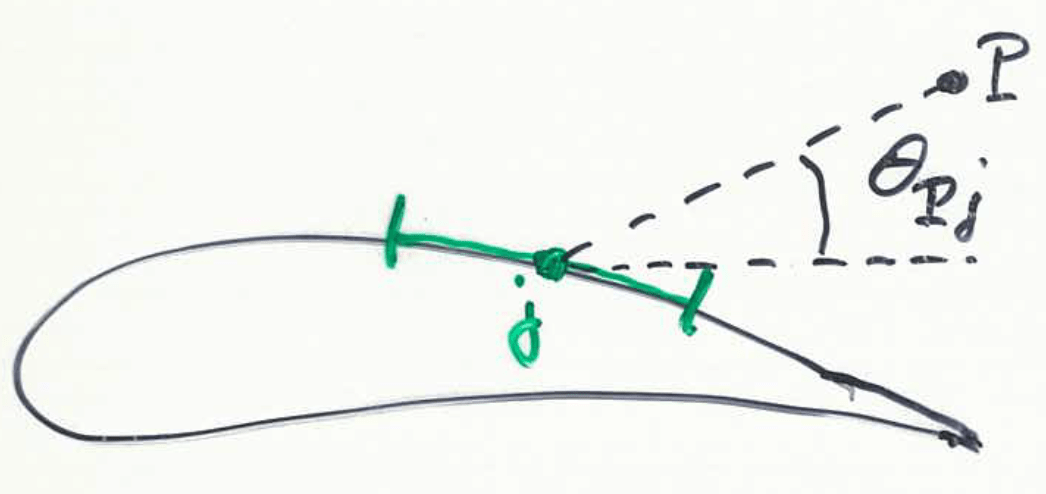
\includegraphics[scale=0.1]{ch2/42}
	\captionof{figure}{}
	\end{wrapfigure}
	This method is similar to the previous one, and since we discussed the thin airfoil theory, we can directly use the definition of the potential function:
	
	\begin{equation}
	U_\infty \cos \alpha x +U_\infty \sin \alpha y - \sum _j \frac{\gamma _j}{2\pi} \int _{\mbox{panel }j} \theta _{jP} \, ds_j.
	\end{equation}
	
	The assumptions made on the previous section are reused here (first order method: intensity constant). The angle $\theta _{jP}$ is the $\theta$-value describing the position of P in a coordinate system centered in the control point of panel j:
	
	\begin{equation}
	\tan \theta _{jP} = \frac{y_P-y_j}{x_P - x_j}.
	\end{equation}
	
	As previously, we compute the vorticity distribution by expressing the condition of null normal potential on the panel:
	
	\begin{equation}
	\frac{\D \phi}{\D n_i} = U_\infty \cos \beta _i - \sum _{j\neq i} \frac{\gamma_j}{2\pi} \int _{\mbox{panel }j} \frac{\D}{\D n_i} (\theta _{ji}) \, ds_j = 0.
	\end{equation}
	
	\begin{wrapfigure}[8]{r}{4cm}
	\vspace{-5mm}
	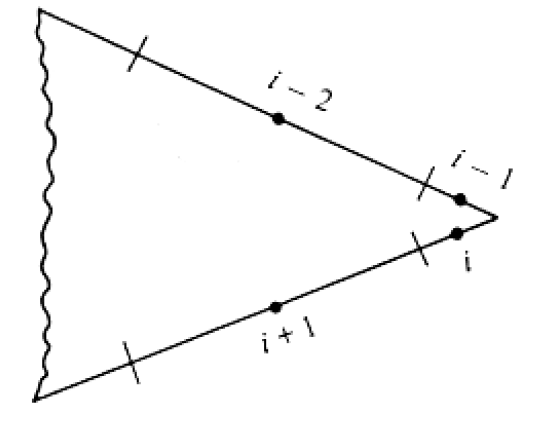
\includegraphics[scale=0.15]{ch2/43}
	\captionof{figure}{}
	\end{wrapfigure}
	Similarly we get a system of N equation of N unknowns. But we have a circulation in this case and we have to satisfy the Kutta condition which states that the vortex distribution on the trailing must be 0. Reffering to the figure, the Kutta condition can be approximated as:
	
	\begin{equation}
	\gamma _{i} = - \gamma _{i-1}.
	\end{equation}
	 
	 With this, we get an overdetermined system of N+1 equations for N unknowns so we can drop one of the panel equation. Once these are solved, we can get the tangential velocity distribution on the body:
	 
	 \begin{equation}
	 v_{ti} = \frac{\D \phi}{\D s_i} = U_\infty \sin \beta _i - \sum _j \frac{\gamma _j}{2\pi} \int _{\mbox{panel }j} \frac{\D}{\D s_i} (\theta_{ji})) \, ds_j = U_\infty \sin \beta _i + \gamma _i.
	 \end{equation}
	 
	 The last $\gamma$ can be understood intuitively. If we remind the previous method, we had a perpendicular velocity on both side of the source panel of intensity $\lambda /2$. Analogously, the vorticies produce a velocity this time tangential to the panel, in opposite direction on both side of the panel, with size $\gamma /2$. The velocity increases with $\gamma$ when moving from one side to the other. Because of the contribution of the other vorticies, there is no flow in the inner part of the panel, but the jump of velocity remains, causing the velocity on the outer side to become $\gamma$. \\
	 
	 The lift is found by using Kutta-Joukowski formula:
	 
	 \begin{equation}
	 \Gamma = \sum _j \gamma _j s_j\qquad \Rightarrow L = \rho _\infty U_\infty \Gamma.
	 \end{equation}
	 
	 Remark: a second order method can be used, choosing the control points on the corner of the panel and postulating a linear variation of the intensity along the panel. In this case the Kutta condition reduces to:
	 
	 \begin{equation}
	 \gamma _1 = 0.
	 \end{equation}
	 
	 \begin{center}
	 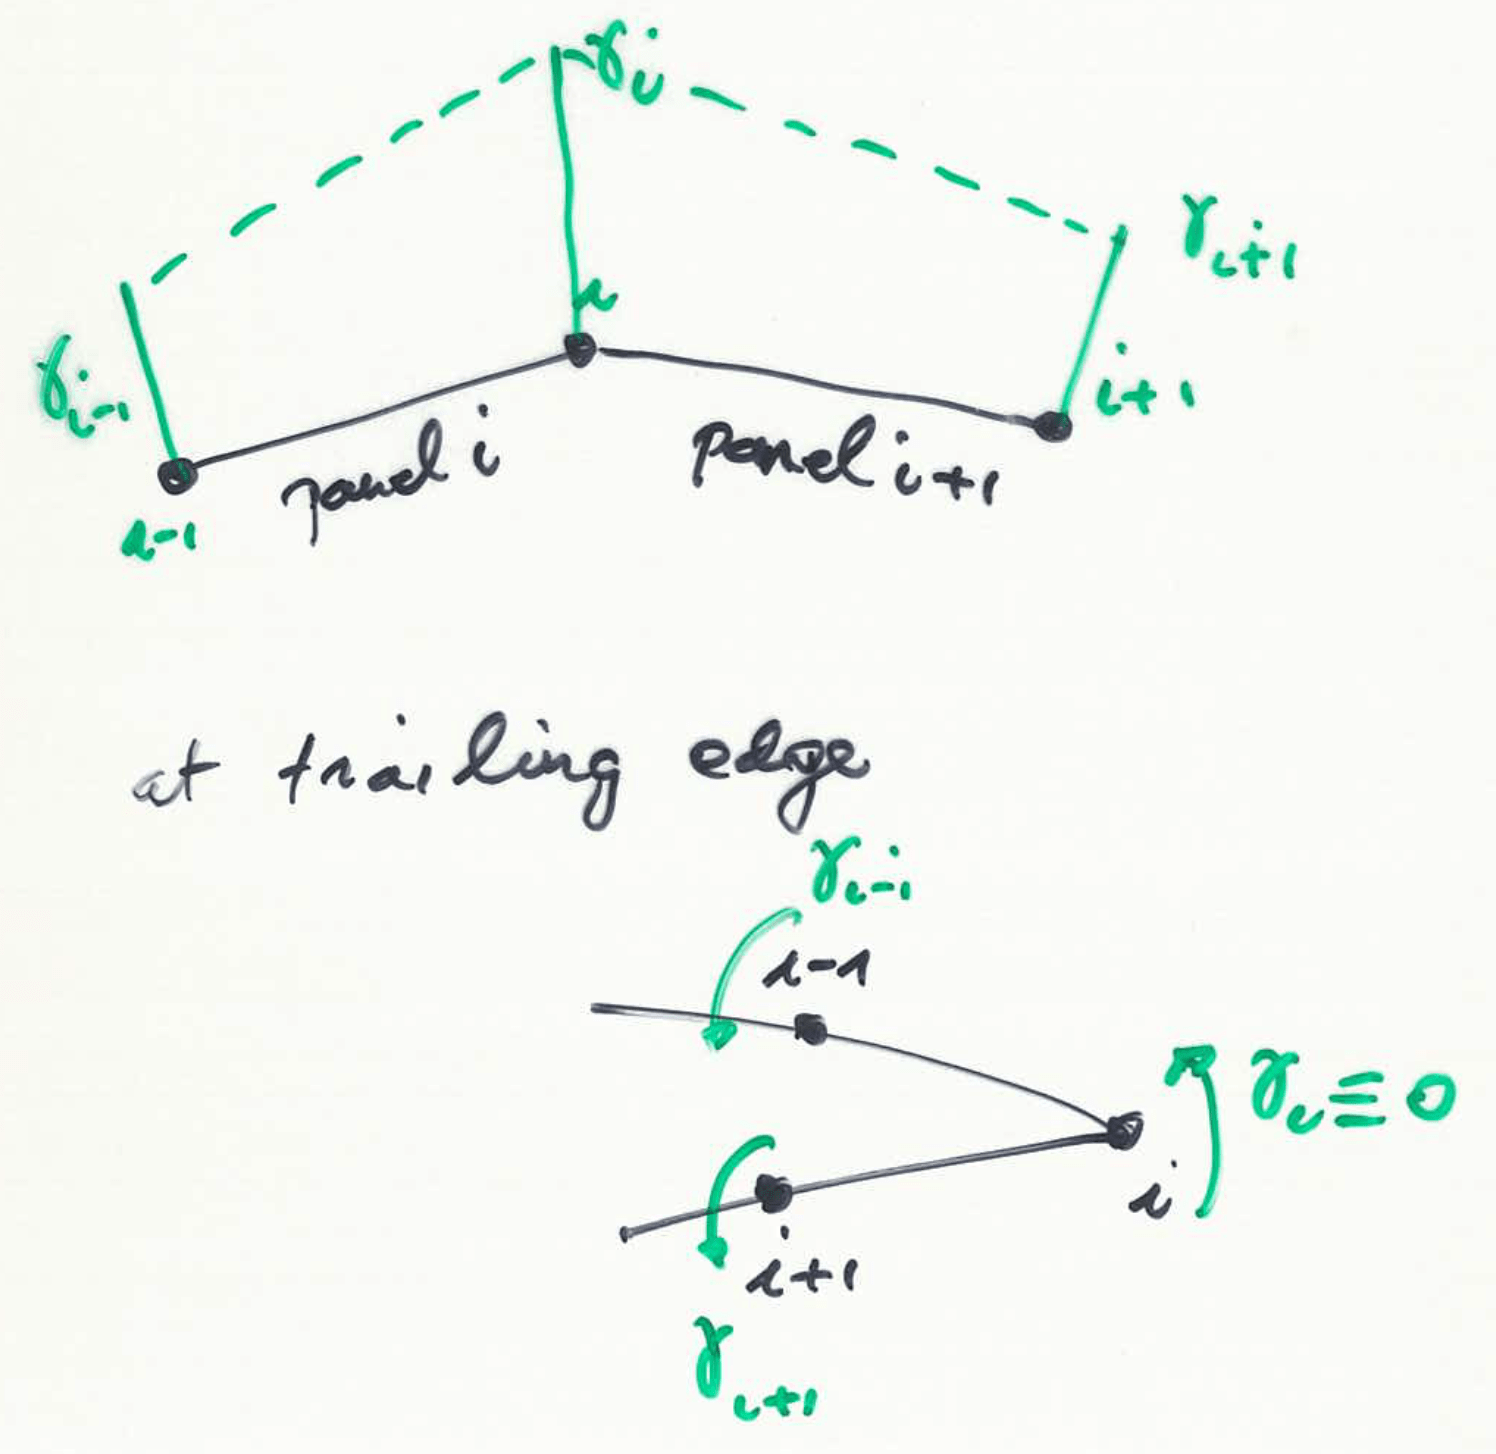
\includegraphics[scale=0.1]{ch2/44}
	 \captionof{figure}{}
	 \end{center}